\documentclass[11pt,a4paper]{article}

\usepackage[margin=2.4cm]{geometry}
\usepackage{amsmath,amssymb}
\usepackage{graphicx}
\usepackage{float}
\usepackage{booktabs}
\usepackage{caption}
\usepackage{subcaption}
\usepackage{siunitx}
\usepackage{xcolor}
\usepackage[colorlinks=true,linkcolor=blue!50!black,citecolor=blue!50!black,urlcolor=blue!50!black]{hyperref}
\usepackage{enumitem}
\usepackage{titlesec}

\captionsetup{font=small,labelfont=bf}
\sisetup{detect-all}
\setlist{nosep,leftmargin=1.4em}
\emergencystretch=3em

\newcommand{\gfour}{Geant4}
\newcommand{\pe}{\ensuremath{N_{\mathrm{pe}}}}
\newcommand{\ngam}{\ensuremath{N_{\gamma}}}

\titleformat{\section}{\large\bfseries}{\thesection}{0.7em}{}
\titleformat{\subsection}{\normalsize\bfseries}{\thesubsection}{0.6em}{}

\title{\vspace{-1.2cm}\bfseries Light Collection in a Polished Plastic Scintillator Read Out by Side-Mounted SiPMs:\\ a \gfour\ Matrix Simulation Study}
\author{J.~Turko}
\date{\today}

\begin{document}
\maketitle

\begin{abstract}
\noindent
We describe a \gfour\ simulation of a \SI{250}{\milli\meter}$\times$\SI{250}{\milli\meter}$\times$\SI{10}{\milli\meter} polished
plastic scintillator (PVT, UPS-92S/EJ-200 class) read out by side-coupled
silicon photomultipliers (SiPMs), modelled on the muon-trigger detector of
Rao \emph{et al.}\ [J.~Appl.\ Phys.\ \textbf{138}, 114504 (2025)]. The detector
is exposed to a vertical \SI{4}{\giga\electronvolt} muon pencil beam. We present
the geometry and the optical-physics implementation in detail---the
\gfour\ \emph{unified} surface model, the finish/type combinations used to
represent four wrapping configurations (bare/black holder, TiO$_2$ paint,
aluminium foil, glossy paper), the photocathode efficiency model that drives
photodetection, and the per-event optical accounting that feeds the analysis.
A \num{48}-file matrix scan (4 SiPM layouts $\times$ 4 reflectors $\times$
3 beam positions, \num{1000} events each) yields collection efficiencies that
reproduce the experimentally observed ordering
$\text{bare} \ll \text{TiO}_2 < \text{Al} \approx \text{glossy}$, with the
absolute scale set by the SiPM photocathode. We report per-event photon yields,
photoelectron spectra, wavelength distributions, and position-resolved
efficiency maps. Two implementation caveats are documented: a rare intermittent
multi-threaded stall in the optical tracking, and a reversed
centre/edge/corner trend in the TiO$_2$ configuration.
\end{abstract}

\tableofcontents
\vspace{0.5em}

% =====================================================================
\section{Introduction and motivation}
% =====================================================================

Plastic scintillators read out at their edges by SiPMs are attractive for
large-area, low-cost muon triggers and veto systems. The amount of scintillation
light that reaches the photosensor is governed almost entirely by how the
non-instrumented faces of the plate are treated: a polished plate in air traps
light by total internal reflection (TIR) and can be a nearly lossless light
guide, whereas a plate wrapped in an absorbing or diffusive material loses
photons at every bounce. Understanding this trade-off quantitatively is the
central design question, and it is precisely where simulation is most useful,
because the photon transport is a multi-bounce random walk that is difficult to
model analytically.

This report documents a \gfour\ (v11.3.2) simulation built to address that
question for the specific geometry and surface treatments of Rao \emph{et
al.}~\cite{Rao2025}. The deliverable is a self-contained ``matrix scan'': every
combination of four SiPM layouts and four reflector treatments, at three beam
positions on the plate. The goal is not to fit a single number but to verify
that the simulation reproduces the \emph{ordering} of light-collection
efficiency that the experiment observes, and to expose the physics behind it.

The remainder of this document is organised as follows.
Section~\ref{sec:detector} describes the detector model.
Section~\ref{sec:physics} details the optical physics implementation, verified
line-by-line against the \gfour\ source.
Section~\ref{sec:sim} covers the simulation workflow and the matrix scan.
Section~\ref{sec:results} presents the results.
Section~\ref{sec:whole} presents the whole-slab full-plate map.
Section~\ref{sec:caveats} documents known caveats.

% =====================================================================
\section{Detector model}
\label{sec:detector}
% =====================================================================

\subsection{Scintillator plate}

The active volume is a rectangular PVT scintillator
$250 \times 250 \times \SI{10}{\milli\meter}$, mirroring the UPS-92S plate of
Ref.~\cite{Rao2025}. It is assigned the \gfour\ NIST base material
\texttt{G4\_PLASTIC\_SC\_VINYLTOLUENE} with a custom optical
properties table~\cite{EJ200,UPS923A}:

\begin{itemize}
  \item refractive index $n = 1.58$ (flat across the visible);
  \item light yield $\SI{1.0e4}{\per\mega\electronvolt}$, single fast component,
        decay time \SI{2.1}{\nano\second}, rise time \SI{0.9}{\nano\second};
  \item emission spectrum peaked at \SI{425}{\nano\meter}
        (\SI{2.917}{\electronvolt}), essentially zero below \SI{380}{\nano\meter}
        and above \SI{550}{\nano\meter};
  \item bulk attenuation length peaked at \SI{3.8}{\meter} and falling steeply
        in the UV to model wavelength-shifter self-absorption;
  \item Birks constant \SI{0.126}{\milli\meter\per\mega\electronvolt}
        (standard PVT value~\cite{Birks1970}).
\end{itemize}

Both scintillation and \v{C}erenkov photons are produced and tracked
(Sec.~\ref{sec:physics}). The optical grid spans \SIrange{310}{700}{\nano\meter}
so that the \v{C}erenkov continuum, which extends well below the scintillation
band, is covered.

\subsection{SiPM readout and coupling}

Each SiPM is modelled mechanically as a $4 \times 4 \times \SI{0.6}{\milli\meter}$
box of ``SiPM epoxy'' ($n = 1.55$), coupled to a side face of the plate through a
\SI{0.1}{\milli\meter} silicone grease pad ($n = 1.46$). The coupling chain is
therefore \emph{scintillator\,$\to$\,grease\,$\to$\,SiPM}, with Fresnel
transmission at each dielectric interface and photodetection at the final
grease/SiPM boundary.

Four layouts are studied (Figs.~\ref{fig:grid1}--\ref{fig:grid4} and the
schematic in Fig.~\ref{fig:layouts}):
\begin{description}
  \item[Config 1 (8 SiPMs)] two SiPMs per side face, at $\pm 50\%$ of the half-length.
  \item[Config 2 (4 SiPMs)] one SiPM per side face, at the \emph{same} $\pm 50\%$
        offsets as config~1---i.e.\ config~1 with one device removed per side,
        the removed slot rotated from side to side so the layout remains
        four-fold symmetric.
  \item[Config 3 (2 SiPMs)] both SiPMs on the \emph{same} face---the top
        ($+y$) edge---at $\pm 50\%$, matching T1/T2 of Ref.~\cite{Rao2025}.
  \item[Config 4 (1 SiPM $+$ WLS clamp)] a single SiPM reading out a
        wavelength-shifting (WLS) fibre clamp along the $-x$ narrow face
        (Sec.~\ref{sec:wls}).
\end{description}
SiPM footprints are clamped so they cannot overhang the slab face.

\begin{figure}[H]
\centering
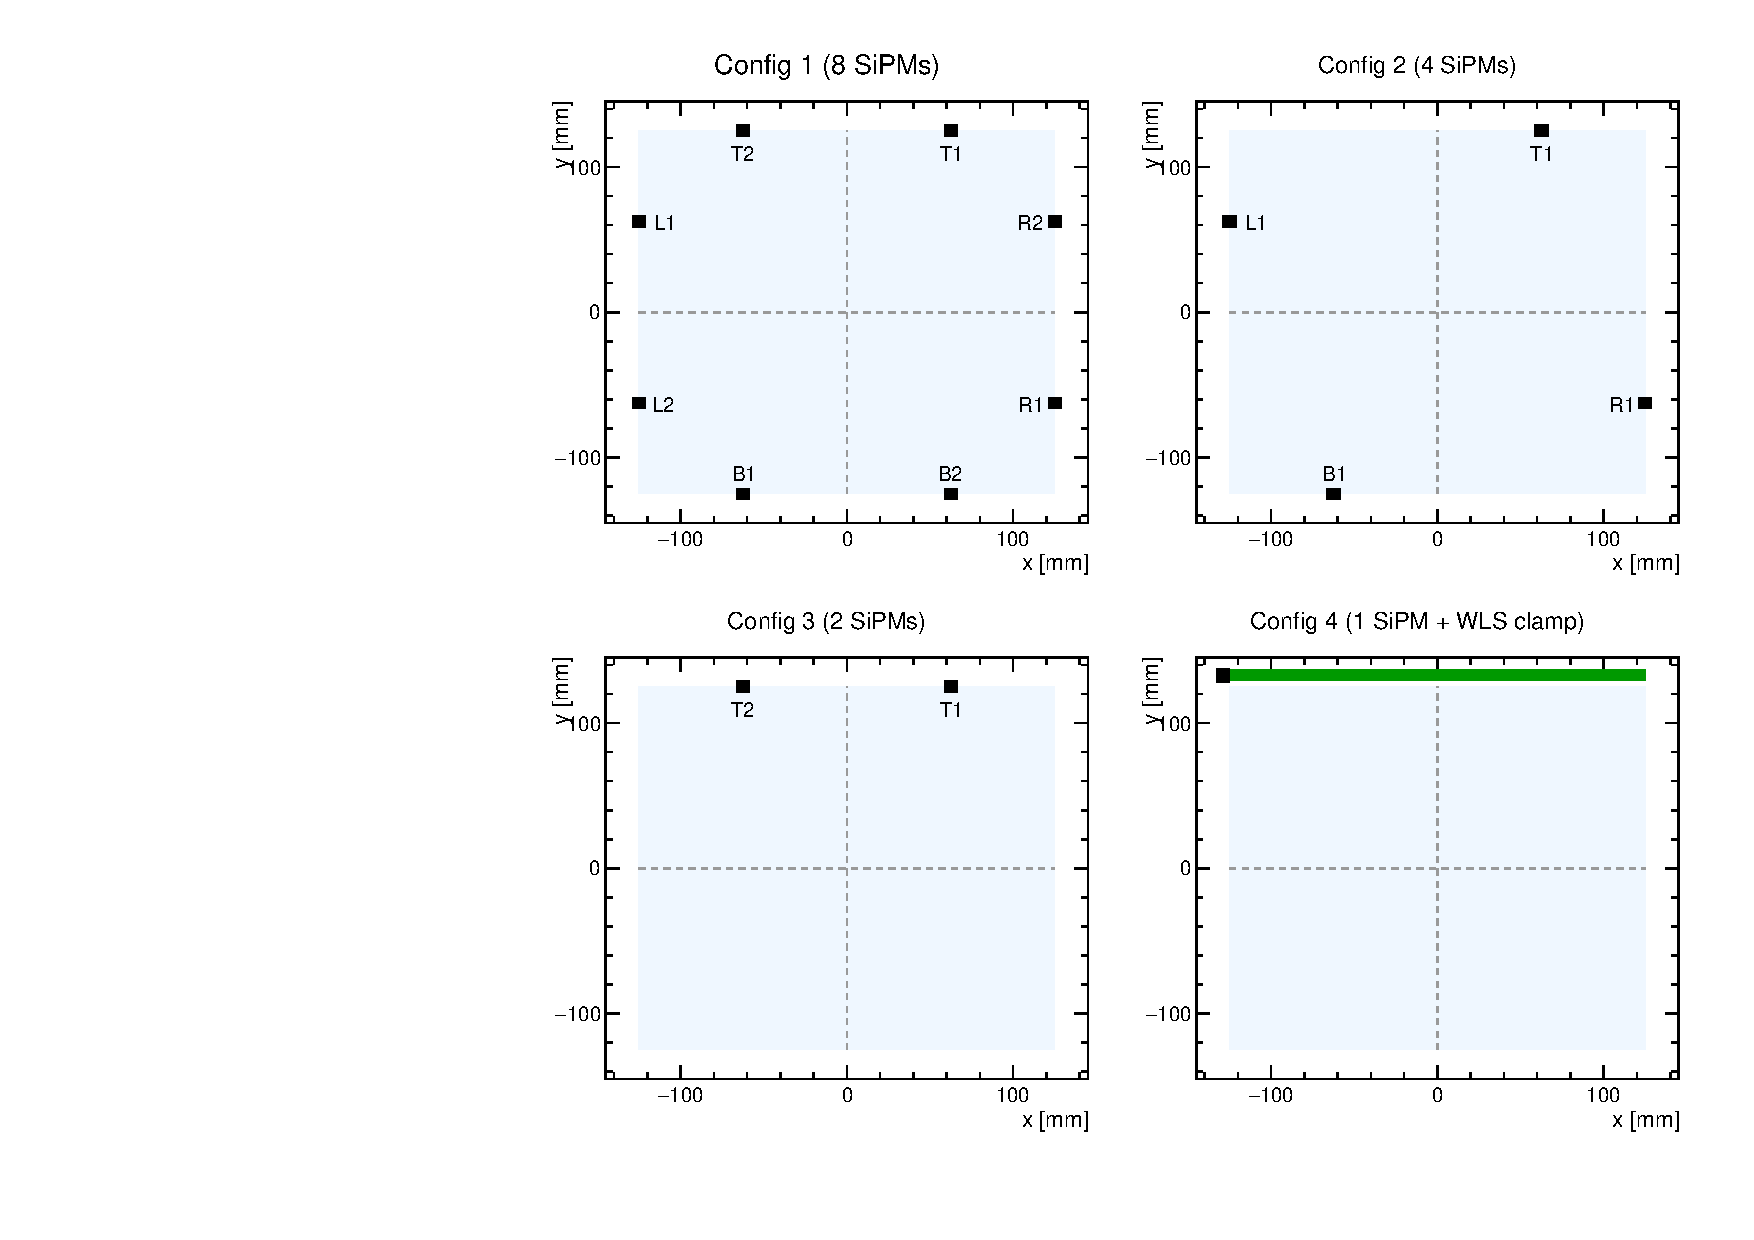
\includegraphics[width=\textwidth]{figures/sipm_layouts.pdf}
\caption{Schematic plan view of the four detector layouts on the
\SI{250}{\milli\meter}$\times$\SI{250}{\milli\meter} plate footprint. Black
squares mark the side-mounted SiPMs (drawn oversized for visibility; the active
area is \SI{4}{\milli\meter}$\times$\SI{4}{\milli\meter}), and the dashed grey
lines are the $x=0$, $y=0$ axes. Config~1 places two SiPMs on each of the four
edges; config~2 places one SiPM per edge at the same offsets as config~1 (one
device removed per side); config~3 places both SiPMs on the top ($+y$) edge;
config~4 uses a single SiPM reading out a WLS fibre clamp, drawn along the top
($+y$) edge with the black read-out SiPM at its left end (green bar), following
Fig.~3(b) of Ref.~\cite{Rao2025}. The inwards-offset labels name the eight
side-mounted sensors (T/B/R/L $=$ top/bottom/right/left); on each edge ``1''
marks the sensor nearer the corner reached when travelling clockwise around
the perimeter, so ``1'' sits at the top-right (T1), bottom-right (R1),
bottom-left (B1) and top-left (L1) corners. This is the scheme used in the
light-sharing discussion below. The same black-square
markers are overlaid on
the collection efficiency maps (Figs.~\ref{fig:grid1}--\ref{fig:grid4}).}
\label{fig:layouts}
\end{figure}

\subsection{Reflector treatments}

Four treatments are applied as a \emph{logical skin} over the non-instrumented
surfaces of the plate; the grease/SiPM patches override the skin locally with
dedicated \emph{border} surfaces. The mapping from the physical treatment to the
\gfour\ optical-surface parameters is the heart of the model and is summarised in
Table~\ref{tab:surfaces} and justified in Sec.~\ref{sec:physics}.

\begin{table}[H]
\centering
\caption{Reflector optical-surface model. All surfaces use the \emph{unified}
model. $R(\lambda)$ is the tabulated reflectivity over
\SIrange{360}{650}{\nano\meter}.}
\label{tab:surfaces}
\footnotesize
\begin{tabular}{@{}llll@{}}
\toprule
Config & \gfour\ type & \gfour\ finish & Key parameters \\
\midrule
Bare / black holder & \texttt{dielectric\_dielectric} & \texttt{polished} (absorber) & $R = T = 0$ (perfect sink) \\
TiO$_2$ paint       & \texttt{dielectric\_dielectric} & \texttt{groundfrontpainted} & Lambertian, $R \approx 0.955$--$0.983$ \\
Aluminium foil      & \texttt{dielectric\_dielectric} & \texttt{polishedbackpainted} & specular spike $=1$, $R \approx 0.84$--$0.91$ \\
Glossy paper        & \texttt{dielectric\_dielectric} & \texttt{polishedbackpainted} & specular spike $=1$, $R \approx 0.90$--$0.955$ \\
\bottomrule
\end{tabular}
\end{table}

A subtle but essential point concerns the \emph{bare} configuration. A
free-standing polished plate is an excellent TIR light guide and would be the
\emph{best} collector---contradicting the measurement, in which the bare plate
gives the weakest signal. The resolution (Sec.~\ref{sec:physics}) is that the
bare plate is clamped into a black 3D-printed holder whose refractive index
($n \approx 1.55$) nearly matches the scintillator's. The faces are then in
\emph{effective optical contact} rather than in contact with air: TIR is
\emph{frustrated}, and light leaks out of the plate into the black walls, where
it is absorbed. This is modelled by a perfect-absorber skin on the plate
($R = T = 0$) for the bare case.

\subsection{Config 4: wavelength-shifting fibre clamp}
\label{sec:wls}

The fourth layout follows the single-SiPM, WLS-readout variant of
Ref.~\cite{Rao2025}. Four \SI{1.0}{\milli\meter}-diameter Kuraray Y-11(200)
wavelength-shifting fibres run the full \SI{250}{\milli\meter} length of the
$-x$ narrow face in a single row. Over most of the length they are parallel at a
\SI{1.5}{\milli\meter} centre-to-centre pitch---so a solid web of clamp material
separates the milled \SI{1.1}{\milli\meter} channels---and converge over the last
\SI{15}{\milli\meter} to a touching \SI{1.0}{\milli\meter} bundle that presents
all four ends to a single \SI{4}{\milli\meter}$\times$\SI{4}{\milli\meter} SiPM at
the $-y$ end; their far $+y$ ends are closed by individual aluminium mirror caps.
A thin \SI{0.10}{\milli\meter} grease film couples the plate face to the clamp,
and each fibre protrudes \SI{0.05}{\milli\meter} through its channel mouth into
that film, keeping the grease continuous against the scintillator. The deliberate
\SI{0.05}{\milli\meter} air annulus between the \SI{1.0}{\milli\meter} fibre and
its \SI{1.1}{\milli\meter} channel is essential: the modelled cladding
($n = 1.49$) exceeds the grease ($n = 1.46$) only marginally, so a snug fit
against the $n \approx 1.55$ clamp would frustrate core--cladding total internal
reflection. The outboard face of the black clamp carries a mirror skin. Because
the core--cladding index step is small, guiding relies on the cladding staying
optically isolated from the clamp, which the air annulus guarantees. The WLS
process is enabled automatically when this geometry is built. In the report's
top-down frame the clamp runs along the \emph{top} edge with the single read-out
SiPM at the \emph{top-left} corner, as in Fig.~3(b) of Ref.~\cite{Rao2025}.
Figure~\ref{fig:viswls} shows an example event in this layout.

\begin{figure}[H]
\centering
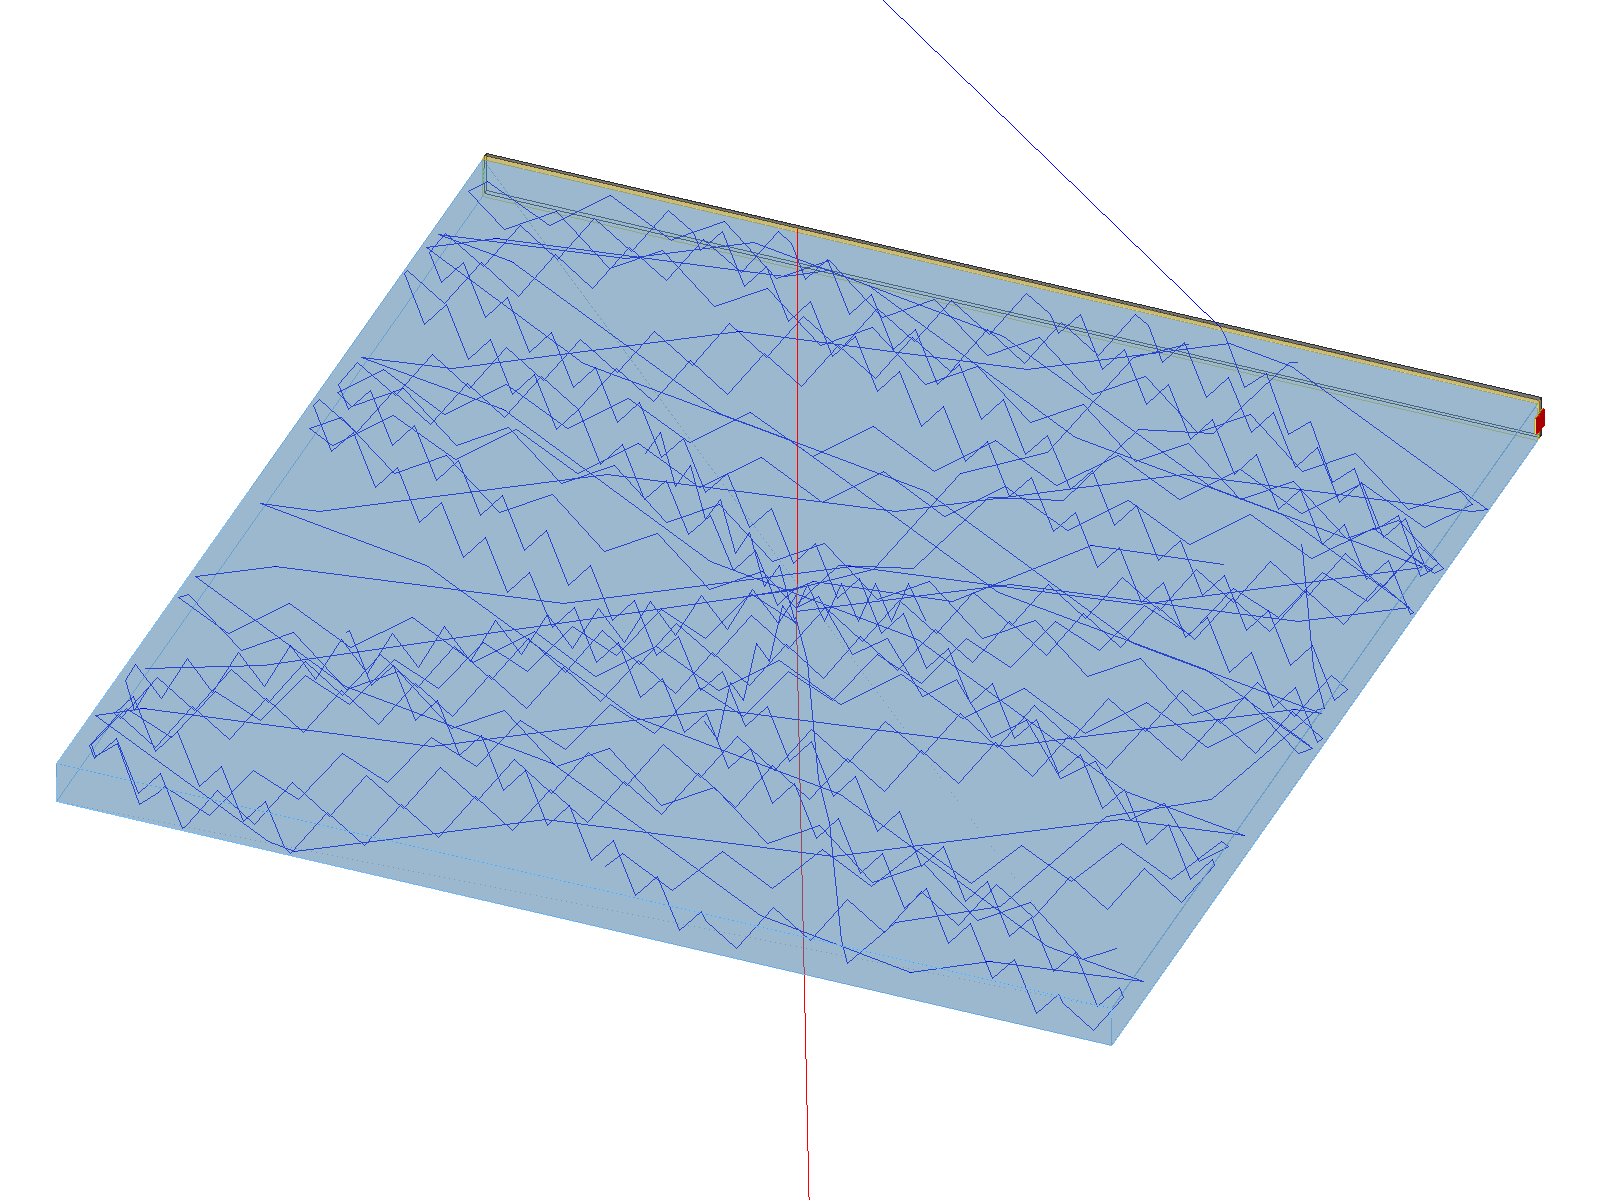
\includegraphics[width=0.75\textwidth]{figures/muon_event_display_wls.png}
\caption{Head-less event display of a single muon in the config-4 WLS-fibre
layout (same visualisation settings as Fig.~\ref{fig:vis}). Scintillation
photons cross the thin grease film into the clamp channels and are
wavelength-shifted in the Y-11 fibre cores, whose re-emission is guided to the
single read-out SiPM at the $-y$ end.}
\label{fig:viswls}
\end{figure}

\begin{figure}[H]
\centering
\begin{subfigure}{0.48\textwidth}
  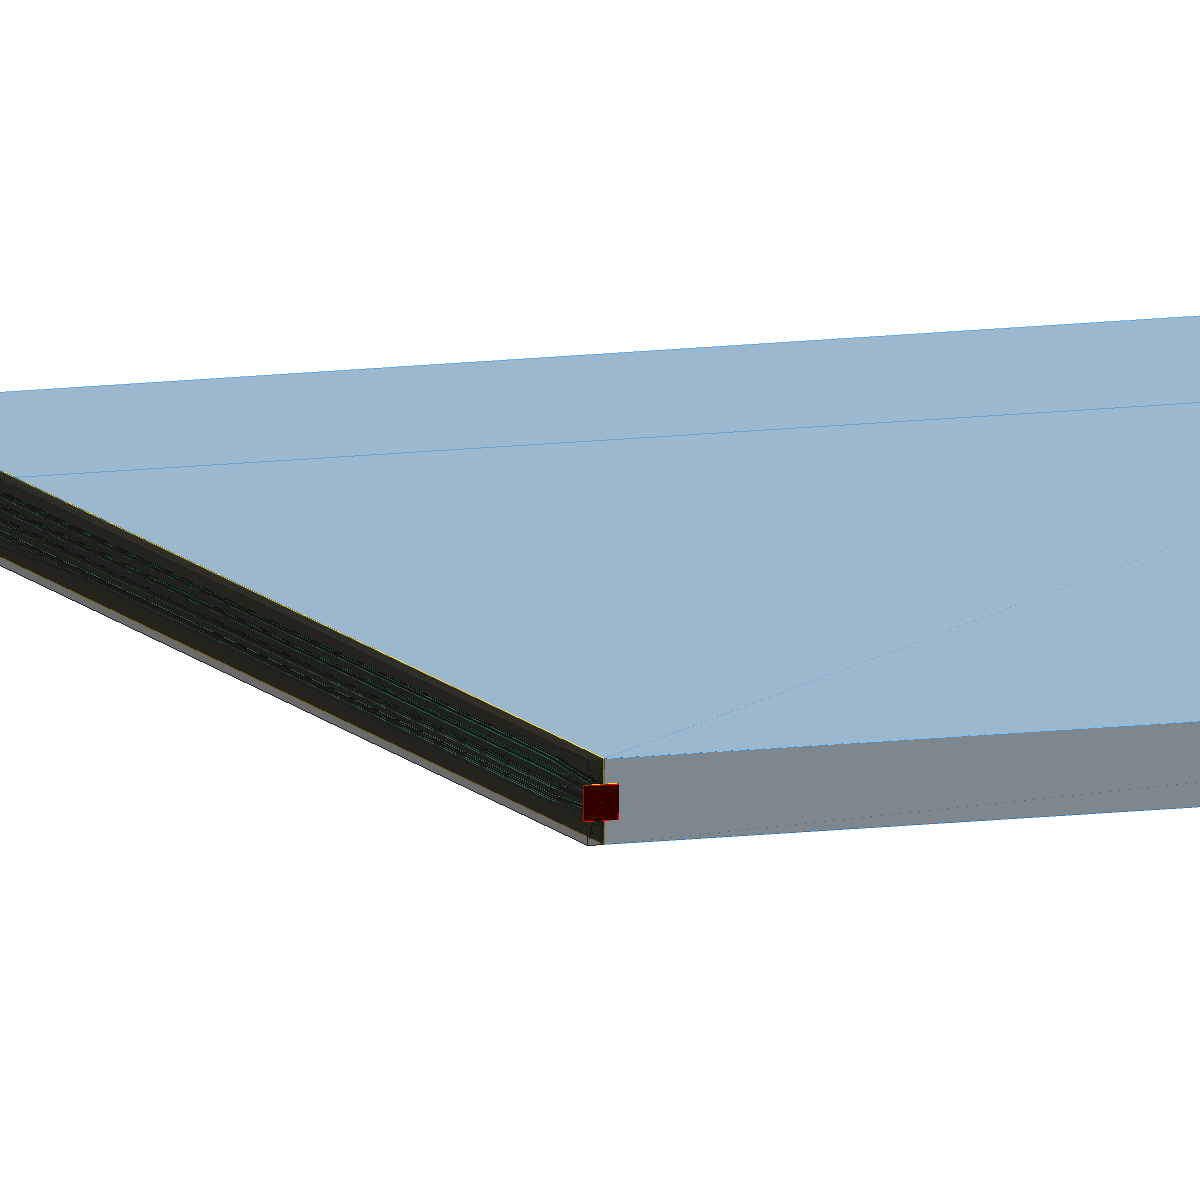
\includegraphics[width=\linewidth]{figures/wls_closeup_overview.png}
  \caption{Overview: the plate with the clamp bar running along its $-x$ face and the read-out sensor at the $-y$ end (report-frame top-left).}
\end{subfigure}\hfill
\begin{subfigure}{0.48\textwidth}
  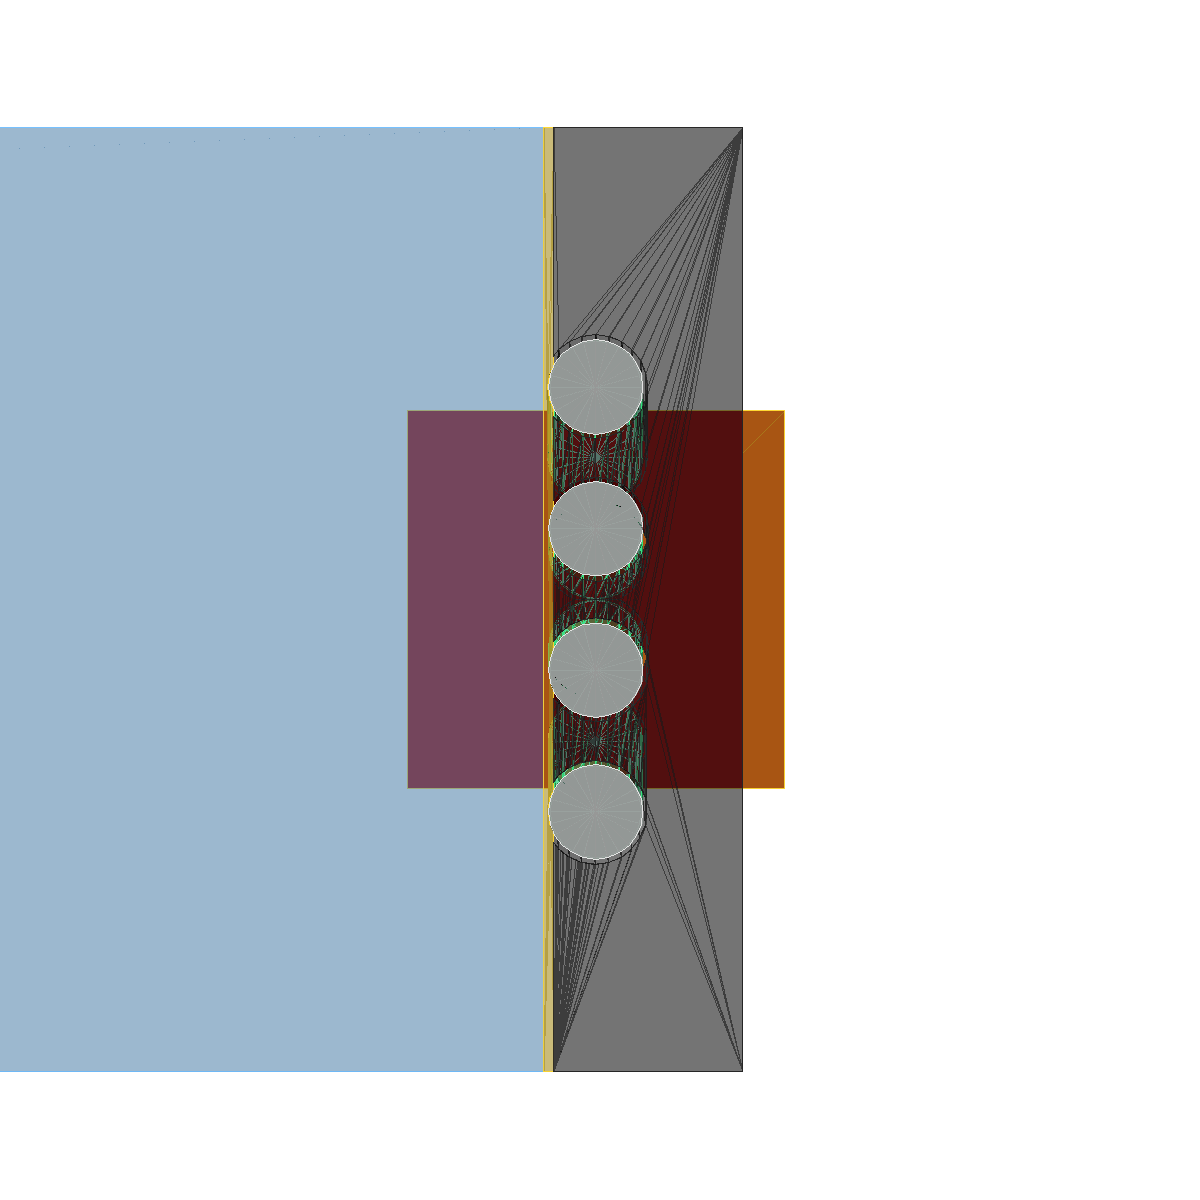
\includegraphics[width=\linewidth]{figures/wls_closeup_xsection.png}
  \caption{Cross-section through the clamp: scintillator (light blue), the thin grease film (amber) in the slab--clamp gap, the four fibre discs (green) seated in their \SI{1.1}{\milli\meter} channels with a \SI{0.05}{\milli\meter} air annulus, and the outboard black clamp.}
\end{subfigure}

\vspace{0.6em}
\begin{subfigure}{0.48\textwidth}
  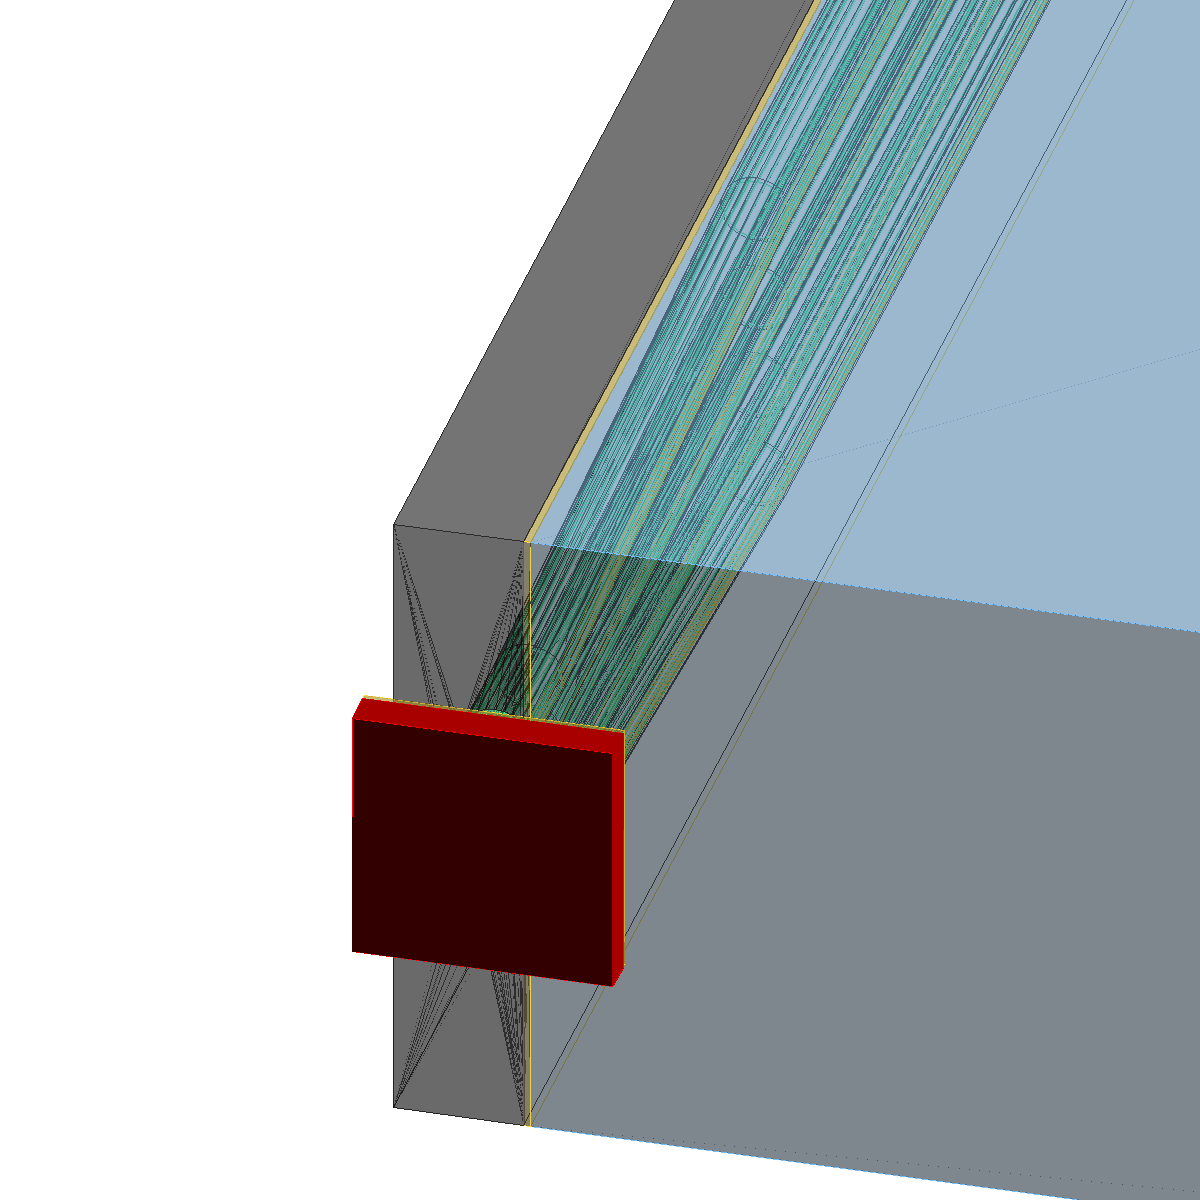
\includegraphics[width=\linewidth]{figures/wls_closeup_readout.png}
  \caption{Read-out end at $-y$: the converged fibre bundle is coupled onto the single SiPM (red).}
\end{subfigure}\hfill
\begin{subfigure}{0.48\textwidth}
  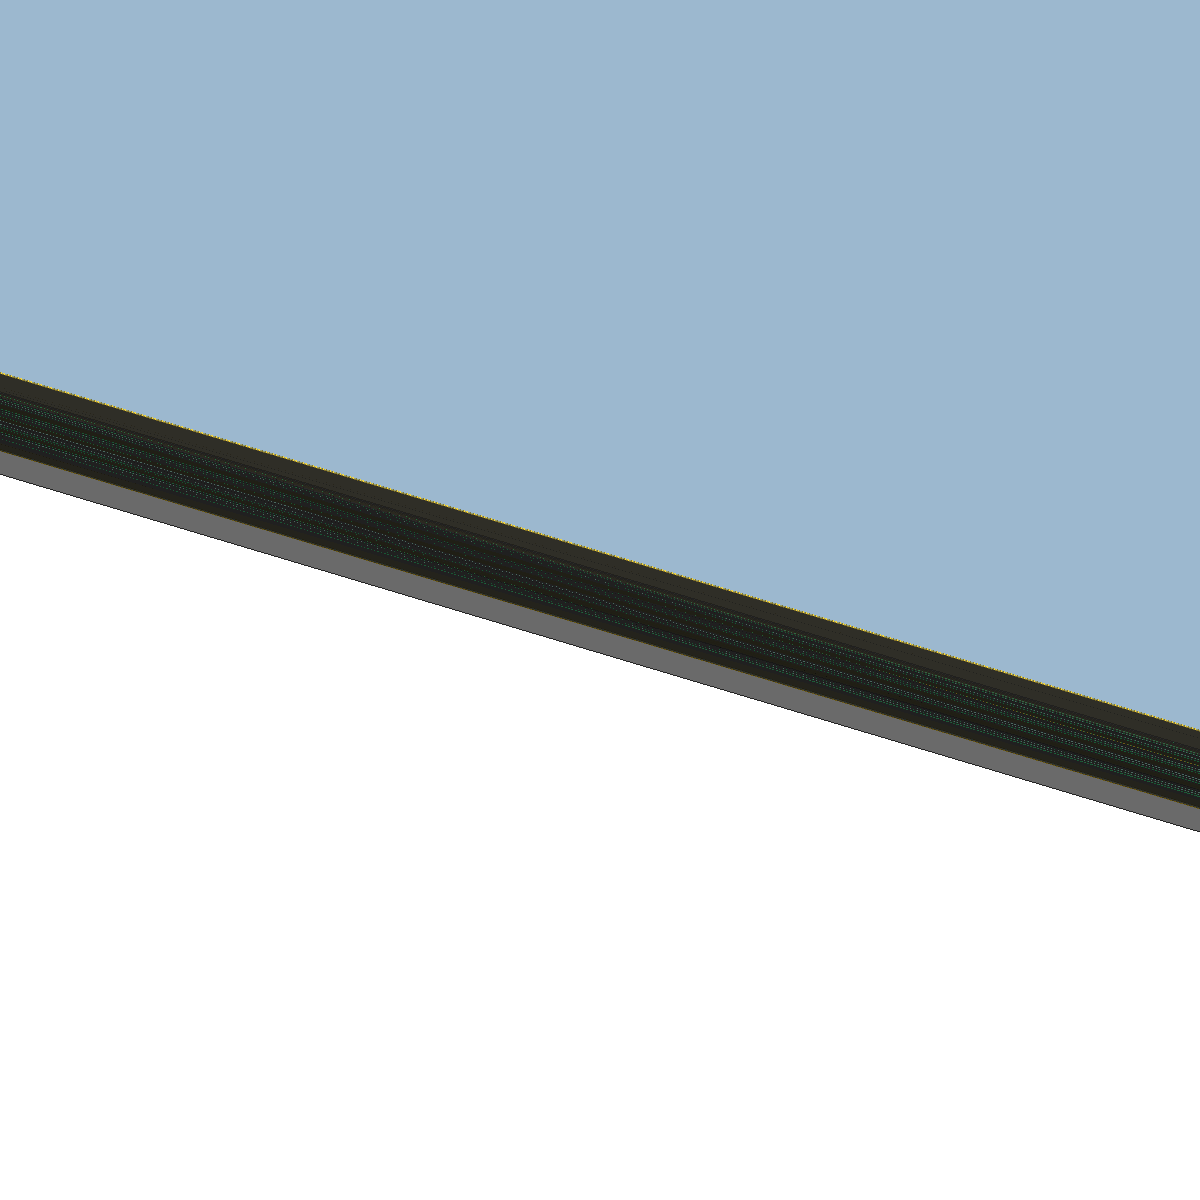
\includegraphics[width=\linewidth]{figures/wls_closeup_length.png}
  \caption{Oblique view of the $-x$ face: the four fibres run the full \SI{250}{\milli\meter} plate length in $y$.}
\end{subfigure}
\caption{Geometry-only close-ups of the config-4 WLS-fibre clamp (\emph{no}
beam-on). Fibre cores are pale green, cladding dark green, the grease film
amber, the black clamp and holder dark grey, and the read-out SiPM red. The four
\SI{1.0}{\milli\meter} fibres sit on the $-x$ narrow face in \SI{1.1}{\milli\meter}
channels separated by clamp webs, with only a thin grease film in the
slab--clamp gap; they converge to a bundle read out at $-y$ by one SiPM and
mirrored at $+y$.}
\label{fig:wlslayout}
\end{figure}

% =====================================================================
\section{Optical physics implementation}
\label{sec:physics}
% =====================================================================

Optical photons are transported by the standard \gfour\ optical physics
module~\cite{G4OpticalPhysics}, with scintillation, \v{C}erenkov, bulk
absorption, Rayleigh scattering and boundary processes all active. Multiple
scattering (Mie) is disabled; wavelength shifting (the \texttt{G4OpWLS} process)
is enabled only for the config-4 fibre layout (Sec.~\ref{sec:wls}) and inert for
all others. This section describes
the boundary physics and the photodetection model, and states explicitly the
\gfour\ behaviour that each modelling choice relies on, verified against the
\gfour\ source in \texttt{.refs/source/processes/optical}.

\subsection{The boundary process and the unified surface model}

Photon crossing of a dielectric interface is handled by
\texttt{G4OpBoundaryProcess}, which selects an \texttt{G4OpticalSurface} from
(\emph{i}) a \texttt{G4LogicalBorderSurface} between two physical volumes or
(\emph{ii}) a \texttt{G4LogicalSkinSurface} on a logical volume. Reading the
source (lines 319--347), the lookup is: a border surface between the pre- and
post-step volumes is consulted first; if none exists, the skin surface of the
daughter (or, failing that, the mother) logical volume is used. This establishes
two facts on which the geometry relies:
\begin{enumerate}
  \item a \texttt{G4LogicalBorderSurface} takes precedence over a
        \texttt{G4LogicalSkinSurface} at the same boundary---hence the grease
        and SiPM patches punch ``holes'' in the wrapping skin;
  \item if no surface object exists at a boundary, the process falls back to
        the default lossless TIR behaviour (via \texttt{DielectricDielectric()}).
\end{enumerate}

The boundary process requires a valid \texttt{RINDEX} on both media; if the
property is absent it sets status \texttt{NoRINDEX} and kills the photon
(lines 289--306, 436--453). Every material in the model therefore carries an
explicit \texttt{RINDEX} table.

For the \emph{unified} model the probability weights for the reflection
sub-models are read from the surface MPT---\texttt{SPECULARSPIKECONSTANT}
($f_{ss}$), \texttt{SPECULARLOBECONSTANT} ($f_{sl}$) and
\texttt{BACKSCATTERCONSTANT} ($f_{bs}$)---together with \texttt{REFLECTIVITY}
(line 381) and, where applicable, \texttt{TRANSMITTANCE} (line 394) and
\texttt{EFFICIENCY} (line 390). The surviving probability
$1 - f_{ss} - f_{sl} - f_{bs}$ is shared between diffuse (Lambertian) and bare
reflection.

\subsection{Reflector finishes}

The four treatments use three distinct code paths in
\texttt{G4OpBoundaryProcess}, which we verified:

\begin{itemize}
  \item \textbf{\texttt{groundfrontpainted}} (TiO$_2$). The finish is handled by
        the ``painted-front'' branch (lines 462--488): a uniform random draw
        against \texttt{REFLECTIVITY} decides absorbed / transmitted / reflected,
        and reflection is set to a pure Lambertian distribution
        (\texttt{LambertianReflection}, line 481). There is \emph{no} TIR at this
        finish---photons are either diffusely reflected or absorbed. This is the
        physically correct description of sub-surface scattering in a thick
        TiO$_2$ paint.
  \item \textbf{\texttt{polishedbackpainted}} (Al, glossy paper). This finish is
        routed to \texttt{DielectricDielectric()} (line 456--459). The
        scintillator/air-gap interface still exhibits Fresnel reflection and TIR;
        sub-critical photons refract into the gap and are returned by the
        backing ``paint'' with reflectivity $R(\lambda)$ and a reflection
        distribution set by $f_{ss}, f_{sl}, f_{bs}$. We choose
        $f_{ss} = 1$ (pure specular spike) for aluminium, since a smooth metal
        foil is a mirror, and likewise for glossy paper---the experimental
        finding that Al $\approx$ glossy and both are the brightest means glossy
        paper is \emph{not} behaving as a diffuser, so it is modelled as a
        slightly lossier mirror than Al.
  \item \textbf{Bare absorber}. This is deliberately \emph{not} a wrapping skin.
        Instead a skin with $R = T = 0$ on the plate (and a matching skin on the
        holder shell) models the frustrated-TIR loss into the black holder.
\end{itemize}

\subsection{Wavelength shifting}
\label{sec:wlphysics}

In the config-4 layout, photons that reach the fibre cores are absorbed and
re-emitted isotropically at longer wavelength by the \texttt{G4OpWLS} process,
which is configured through the fibre material's \texttt{WLSABSLENGTH},
\texttt{WLSCOMPONENT} and \texttt{WLSTIMECONSTANT} properties (Y-11 absorption
peaks near \SI{430}{\nano\meter}, re-emission near \SI{490}{\nano\meter}). The
process is switched on by the physics list when the WLS geometry is detected (the
\gfour\ optical-physics constructor reads the process activation at build time,
so the flag is set before the base construction). Because the shifted emission no
longer overlaps the fibre absorption band, the re-emitted light is transported
losslessly along the fibre by TIR to the read-out SiPM---which is why the
detected config-4 spectrum is green-shifted (mean $\sim\!\SI{496}{\nano\meter}$)
relative to the direct-coupled configurations.

\subsection{Photodetection: the SiPM photocathode}

Photodetection is delegated entirely to \gfour, rather than being drawn
manually in the sensitive detector. The grease/SiPM boundary is a
\texttt{dielectric\_metal} surface whose MPT carries the SiPM
\texttt{EFFICIENCY} as a function of photon energy, i.e.\ the photon detection
efficiency (PDE) of an ASD-NUV4S-P-40 device, peaking at $\approx 0.43$ near
\SI{420}{\nano\meter}, with \texttt{REFLECTIVITY} $=0$.

The mechanism is worth stating precisely because it is the reason the sensitive
detector needs no random draw of its own. In \texttt{DielectricMetal()}
(lines 724--817), when the Fresnel--PDE roll places a photon in the ``absorbed''
channel, \texttt{DoAbsorption()} is called. Inside it (header, lines 305--320):
\begin{equation}
  f_{\mathrm{status}} =
  \begin{cases}
    \mathrm{Absorption}, & \xi \ge \operatorname{EFFICIENCY}(\lambda),\\[2pt]
    \mathrm{Detection},  & \xi <  \operatorname{EFFICIENCY}(\lambda),
  \end{cases}
  \qquad \xi \sim U(0,1),
\end{equation}
where $\operatorname{EFFICIENCY}(\lambda)$ is the tabulated PDE. The absorbed
photon is assigned a non-zero
\texttt{LocalEnergyDeposit} \emph{only} when the PDE draw succeeds. Back in
\texttt{PostStepDoIt}, if the status is \texttt{Detection} \emph{and} the
invoke-SD flag is set, the sensitive detector is invoked (lines 559--560):
\begin{equation}
  f_{\mathrm{status}} = \mathrm{Detection}\ \wedge\ f_{\mathrm{InvokeSD}}
  \ \Longrightarrow\ \operatorname{InvokeSD}(\text{step}).
\end{equation}
The flag is enabled in the physics list via
\texttt{G4OpticalParameters::SetBoundaryInvokeSD(true)}. Consequently the
sensitive-detector \texttt{ProcessHits} fires \emph{only} for genuine
photoelectrons (it tests that the step energy deposit is positive), counts one
\pe{} per call, and kills the photon (the SiPM is opaque). This is a clean
separation of concerns: the physics of the photocathode lives in the optical
surface, and the sensitive detector only books hits.

\subsection{Per-event optical accounting}

A thread-local diagnostic record (\texttt{OpticalDiag}) accumulates, per event:
scintillation photons, \v{C}erenkov photons, terminated photons, detected
photoelectrons, and photons that escaped to the world. The primary muon's
first-entry position in the slab is captured on the first step inside the
scintillator logical volume and stored in slab-local coordinates. At end of
event the sensitive detector writes one row per (event, SiPM), \emph{including
zero-detection rows}, so the sample is unbiased in the muon interaction
position. Each row carries the entry position, the event's produced-photon
count (the efficiency denominator), the detected count in that SiPM, the first
arrival time, the mean and RMS detected wavelength, and the track weight. This
one tree supports per-SiPM, combined, and spatially-binned collection-efficiency
analyses.

Figure~\ref{fig:vis} shows a head-less event display of a single vertical muon
in the glossy-wrapped plate (config~1). For legibility the display uses a
\SI{30}{\mega\electronvolt} muon---just below the \v{C}erenkov threshold of the
scintillator---with the scintillation yield rescaled, so that the individual
optical tracks can be followed: photons are generated along the muon path,
propagate by total internal reflection and specular reflection off the wrapper,
and terminate on the SiPM patches at the four edges.

\begin{figure}[H]
\centering
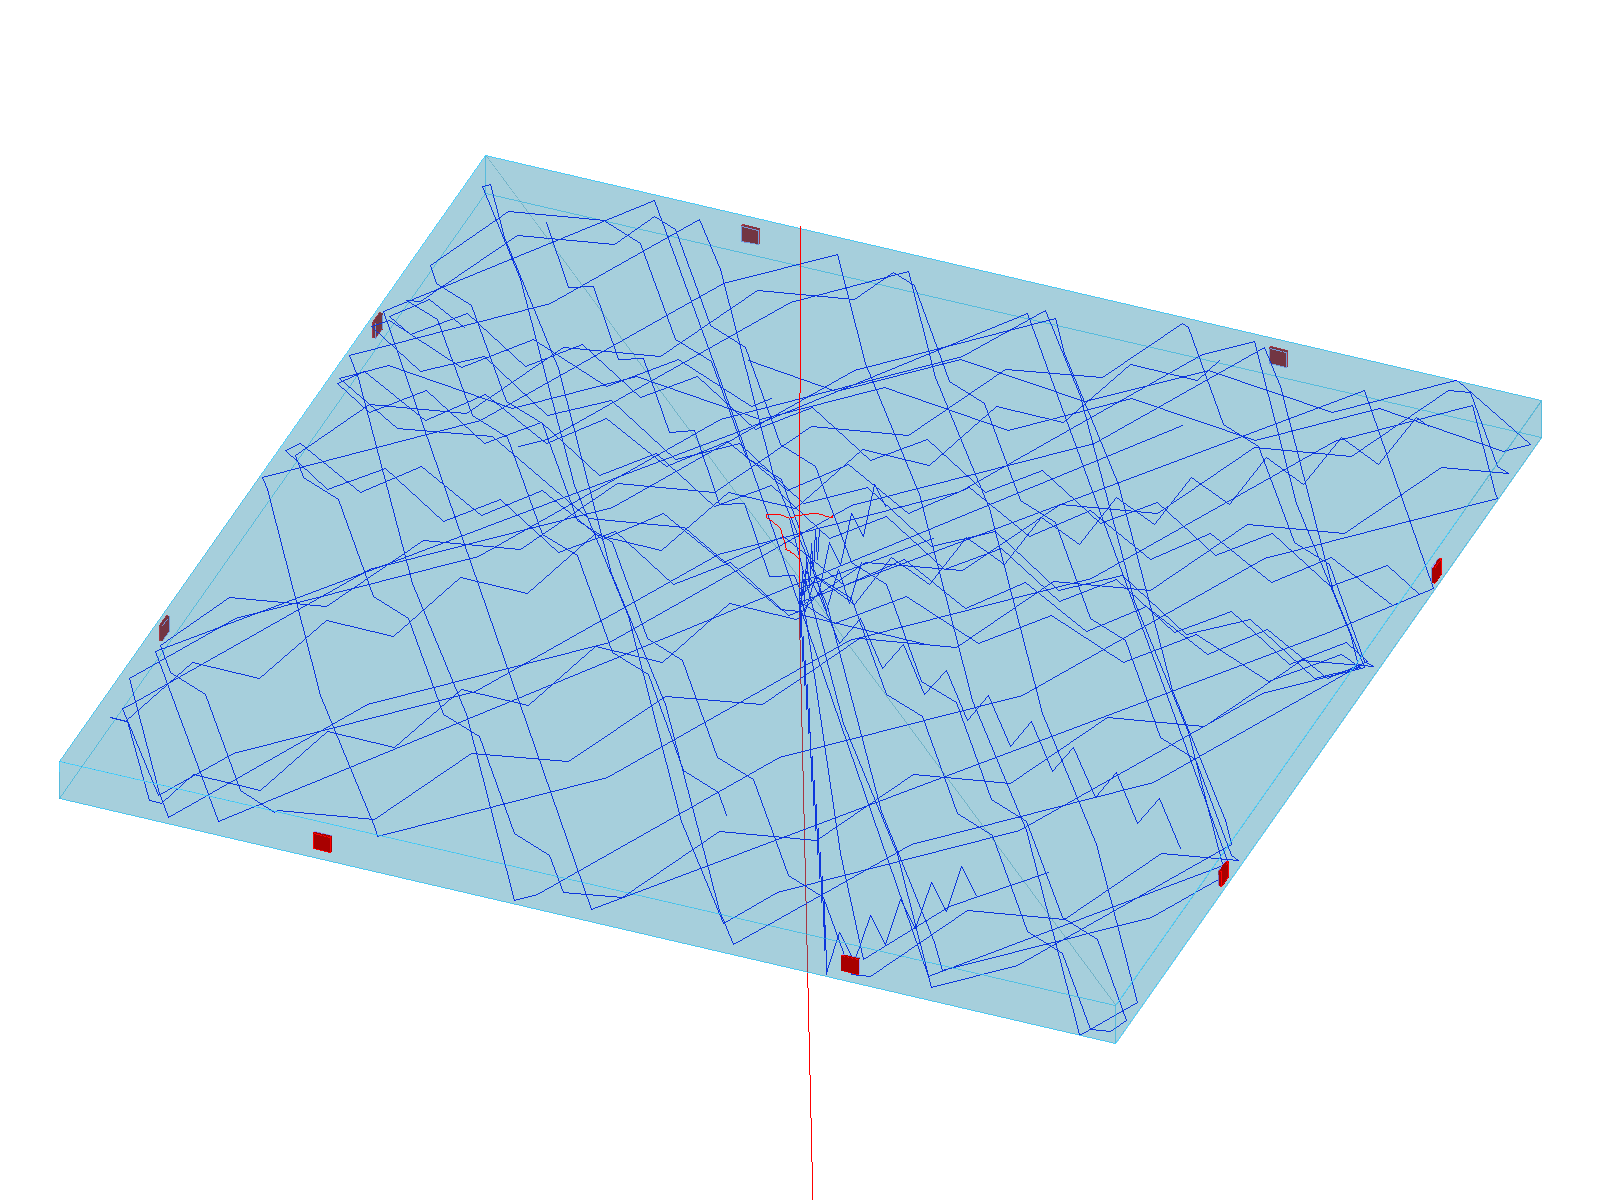
\includegraphics[width=0.75\textwidth]{figures/muon_event_display.png}
\caption{Head-less (\texttt{TSG\_OFFSCREEN}) event display of one vertical muon
in the glossy-wrapped plate with the config-1 layout, on a white background. The
red line is the muon and the blue lines are optical photons (here purely
scintillation, since the muon is below the \v{C}erenkov threshold); the plate and
its reflective wrapper are drawn as translucent surfaces with their edges
outlined, and the SiPMs are opaque red.
Both the muon energy (\SI{30}{\mega\electronvolt}, below the \v{C}erenkov
threshold) and the photon yield are chosen for visualisation only, so that
individual tracks are resolved rather than merging into a saturated blob. The
display is generated reproducibly by \texttt{macros/muon\_vis.mac}.}
\label{fig:vis}
\end{figure}

% =====================================================================
\section{Simulation setup and matrix scan}
\label{sec:sim}
% =====================================================================

The primary source is a vertical muon pencil beam: a \SI{50}{\milli\meter}$\times$\SI{50}{\milli\meter}
square beam of \SI{4}{\giga\electronvolt} $\mu^-$ normally incident on the plate,
with the beam centre placed at three positions, each irradiating a
\SI{50}{\milli\meter}$\times$\SI{50}{\milli\meter} patch lying \emph{entirely
on} the polished plate. With the plate spanning $[-125,125]\,\si{\milli\meter}$
in both $x$ and $y$, the patch centres are
\[
  \text{centre} = (0,0),\qquad
  \text{edge} = (0,-100),\qquad
  \text{corner} = (100,-100)\ \si{\milli\meter},
\]
so the illuminated regions are $[-25,25]^2$, $[-25,25]\times[-125,-75]$ and
$[75,125]\times[-125,-75]$ respectively (report frame: $+y$ is the top,
$-x$ the left). This places the edge and corner regions on the bottom
($-y$) edge, opposite the single instrumented face of config~3 (top, $+y$),
as in Fig.~3 of Ref.~\cite{Rao2025}. It also matches the \SI{50}{\milli\meter}$\times$\SI{50}{\milli\meter}
active area of the muon coincidence detector (MCD) that defines the regions of
interest in Ref.~\cite{Rao2025}, and keeps the irradiated area---and hence the
denominator of Eq.~\ref{eq:eff}---equal at all three positions. Each
(config, reflector, position) runs \num{1000} events after a single
\texttt{/run/initialize}. The matrix therefore comprises
\[
  4\ \text{configs} \times 4\ \text{reflectors} \times 3\ \text{positions}
  = 48\ \text{files}, \qquad 48 \times \num{1000} = \num{48000}\ \text{events}.
\]

Runs used \num{8} threads on an 8-thread (\num{4}-physical-core) workstation.
The optional per-slab optical track-length flux map is disabled for the matrix
(it is retained as a separate diagnostic); the collection efficiency is
reconstructed entirely offline from the \texttt{sipmHits} tree at any desired
binning, so the map is not needed.

\begin{figure}[H]
\centering
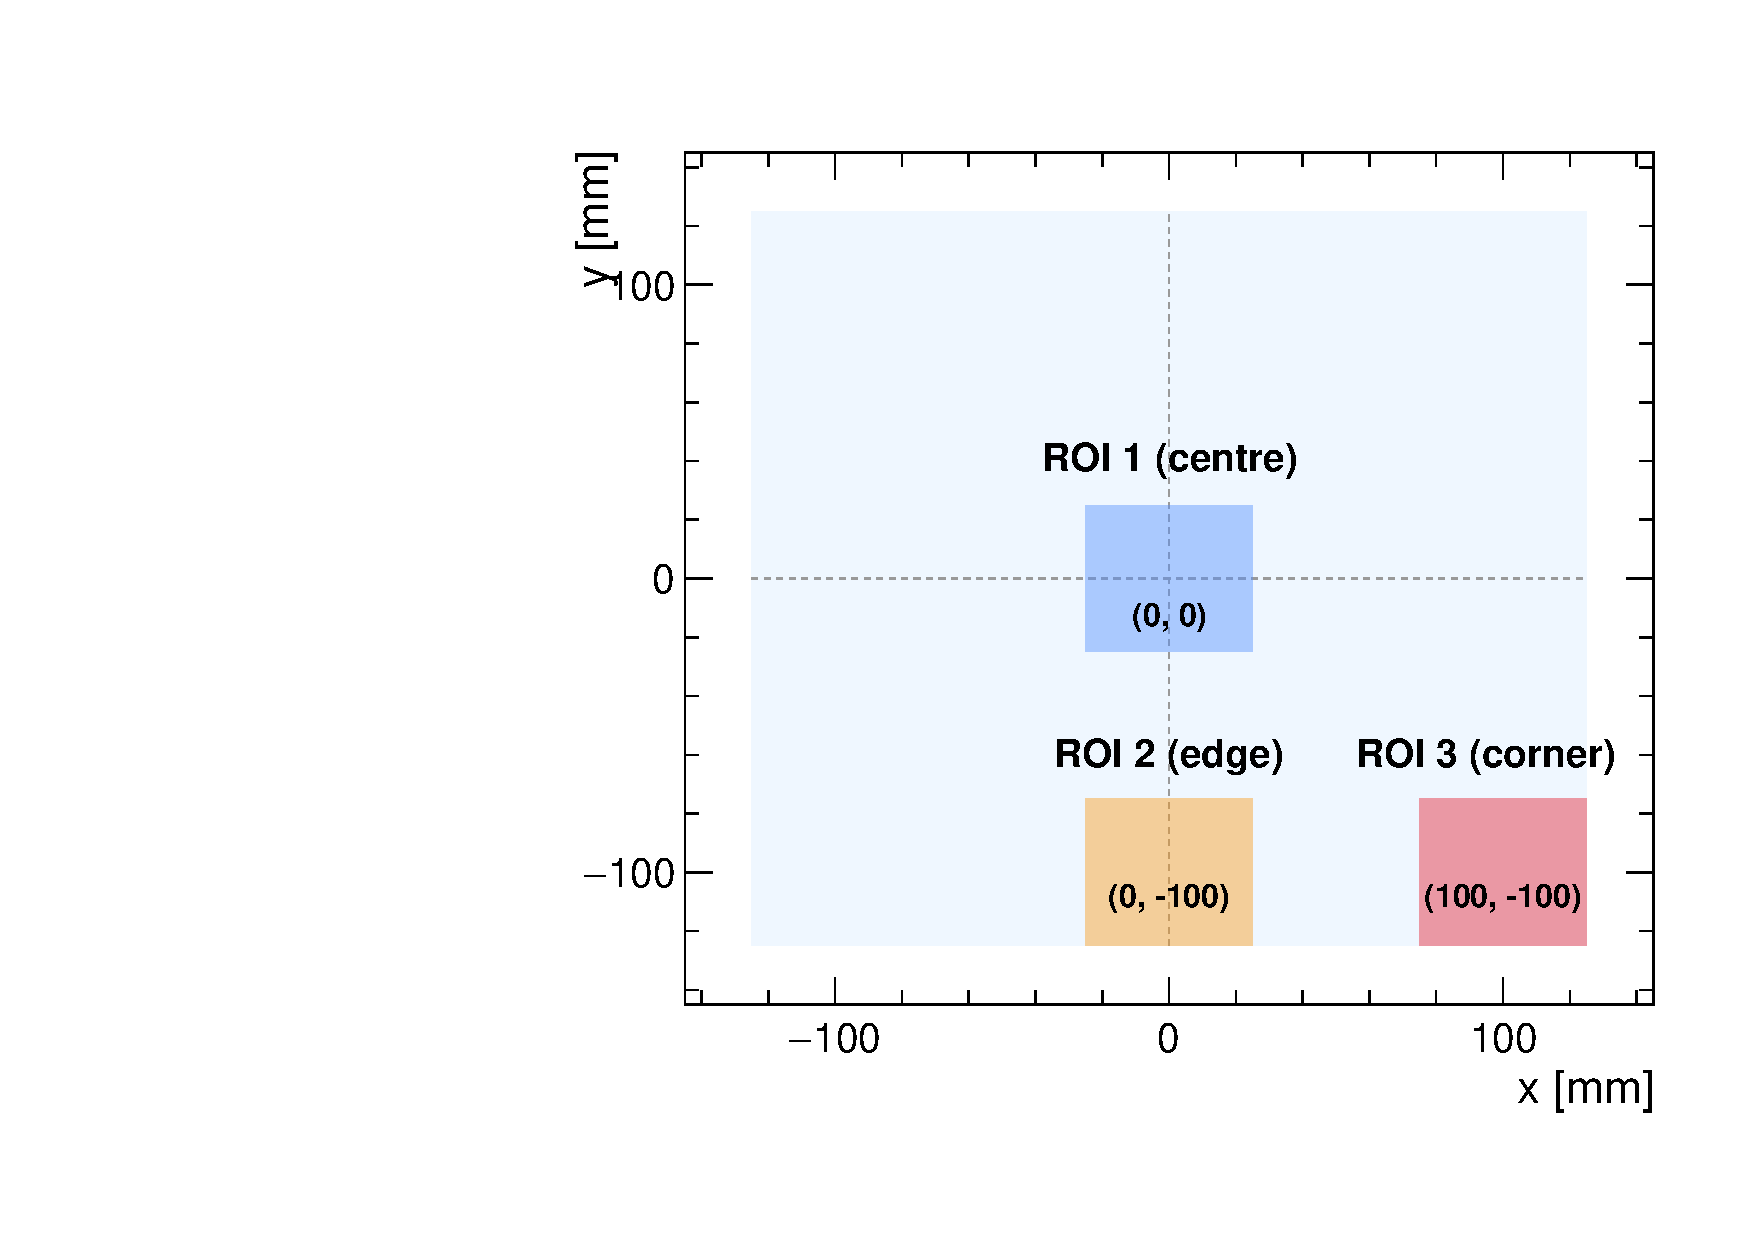
\includegraphics[width=0.55\textwidth]{figures/irradiation_sites.pdf}
\caption{Plan view of the three irradiation sites (regions of interest) on the
\SI{250}{\milli\meter}$\times$\SI{250}{\milli\meter} plate, in the report frame
($+y$ top, $-x$ left). Each coloured square is the \SI{50}{\milli\meter}$\times$\SI{50}{\milli\meter}
footprint of the vertical muon beam: ROI~1 (centre, blue) at $(0,0)$,
ROI~2 (edge, orange) at $(0,-100)$, and ROI~3 (corner, red) at $(100,-100)$.
The edge and corner sites lie on the bottom ($-y$) edge, opposite the
single instrumented face of config~3.}
\label{fig:irr}
\end{figure}

The collection efficiency is defined, for a set $\mathcal{S}$ of SiPMs and an
event $e$, as
\begin{equation}
  \varepsilon = \frac{\displaystyle\sum_{e}\sum_{s\in\mathcal{S}} \pe^{(e,s)}}
                     {\displaystyle\sum_{e}\ngam^{(e)}},
  \label{eq:eff}
\end{equation}
where $\ngam^{(e)}$ is the total number of optical photons generated in the slab
during event $e$ (scintillation plus \v{C}erenkov) and $\pe^{(e,s)}$ is the
number of photoelectrons in SiPM $s$. The all-SiPM sum over the three beam
positions is quoted as the figure of merit.

For presentation, all position-resolved results (the maps of
Figs.~\ref{fig:irr} and \ref{fig:grid1}--\ref{fig:grid4} and the whole-slab maps
of Sec.~\ref{sec:whole}) are shown in the report frame with the top edge at $+y$,
the bottom at $-y$, the left at $-x$ and the right at $+x$. The internal
simulation frame is this view rotated by \SI{90}{\degree} clockwise; the primary
muon entry points and the SiPM markers are mapped into the report frame by
$(x,y)\to(y,-x)$ before plotting. This rotation is a rigid change of view and
leaves every scalar result (yields, spectra, efficiencies) unchanged; it only
fixes the orientation of config~3 (top edge) and of the edge/corner irradiation
sites (bottom edge).

% =====================================================================
\section{Results}
\label{sec:results}
% =====================================================================

\subsection{Overall collection efficiency}

Figure~\ref{fig:bars} shows the overall collection efficiency
(Eq.~\ref{eq:eff}, all SiPMs, all three beam positions pooled) for every
(config, reflector) pair, and Table~\ref{tab:eff} lists the numbers. The
ordering
\[
  \text{bare}\ (6\times10^{-6}\text{--}2\times10^{-4})\ \ll\
  \text{TiO}_2\ (2\times10^{-4}\text{--}10^{-2})
  \ <\ \text{Al}\ (1.4\text{--}2.6\times10^{-2})
  \ \approx\ \text{glossy}\ (1.5\text{--}3.0\times10^{-2})
\]
holds for all four layouts, reproducing the experimental result of
Ref.~\cite{Rao2025}. The bare configuration is suppressed by two to three orders
of magnitude, as required by the frustrated-TIR absorber model: without a
reflective wrap, the trapped light is lost to the black holder. Al and glossy
paper are statistically indistinguishable within the \num{1000}-event-per-position
sample and are the best collectors. Four SiPMs on four faces (config~2)
outperform two SiPMs on one face (config~3), and the eight-SiPM layout
(config~1) gives the highest efficiency, as expected from the larger
photosensitive coverage. The single-SiPM WLS-fibre layout (config~4) collects
substantially less than the direct-coupled layouts: only the fraction of light
that reaches the fibre face is wavelength-shifted and guided to the sensor, so
its efficiency sits about an order of magnitude below config~3.

\begin{figure}[H]
\centering
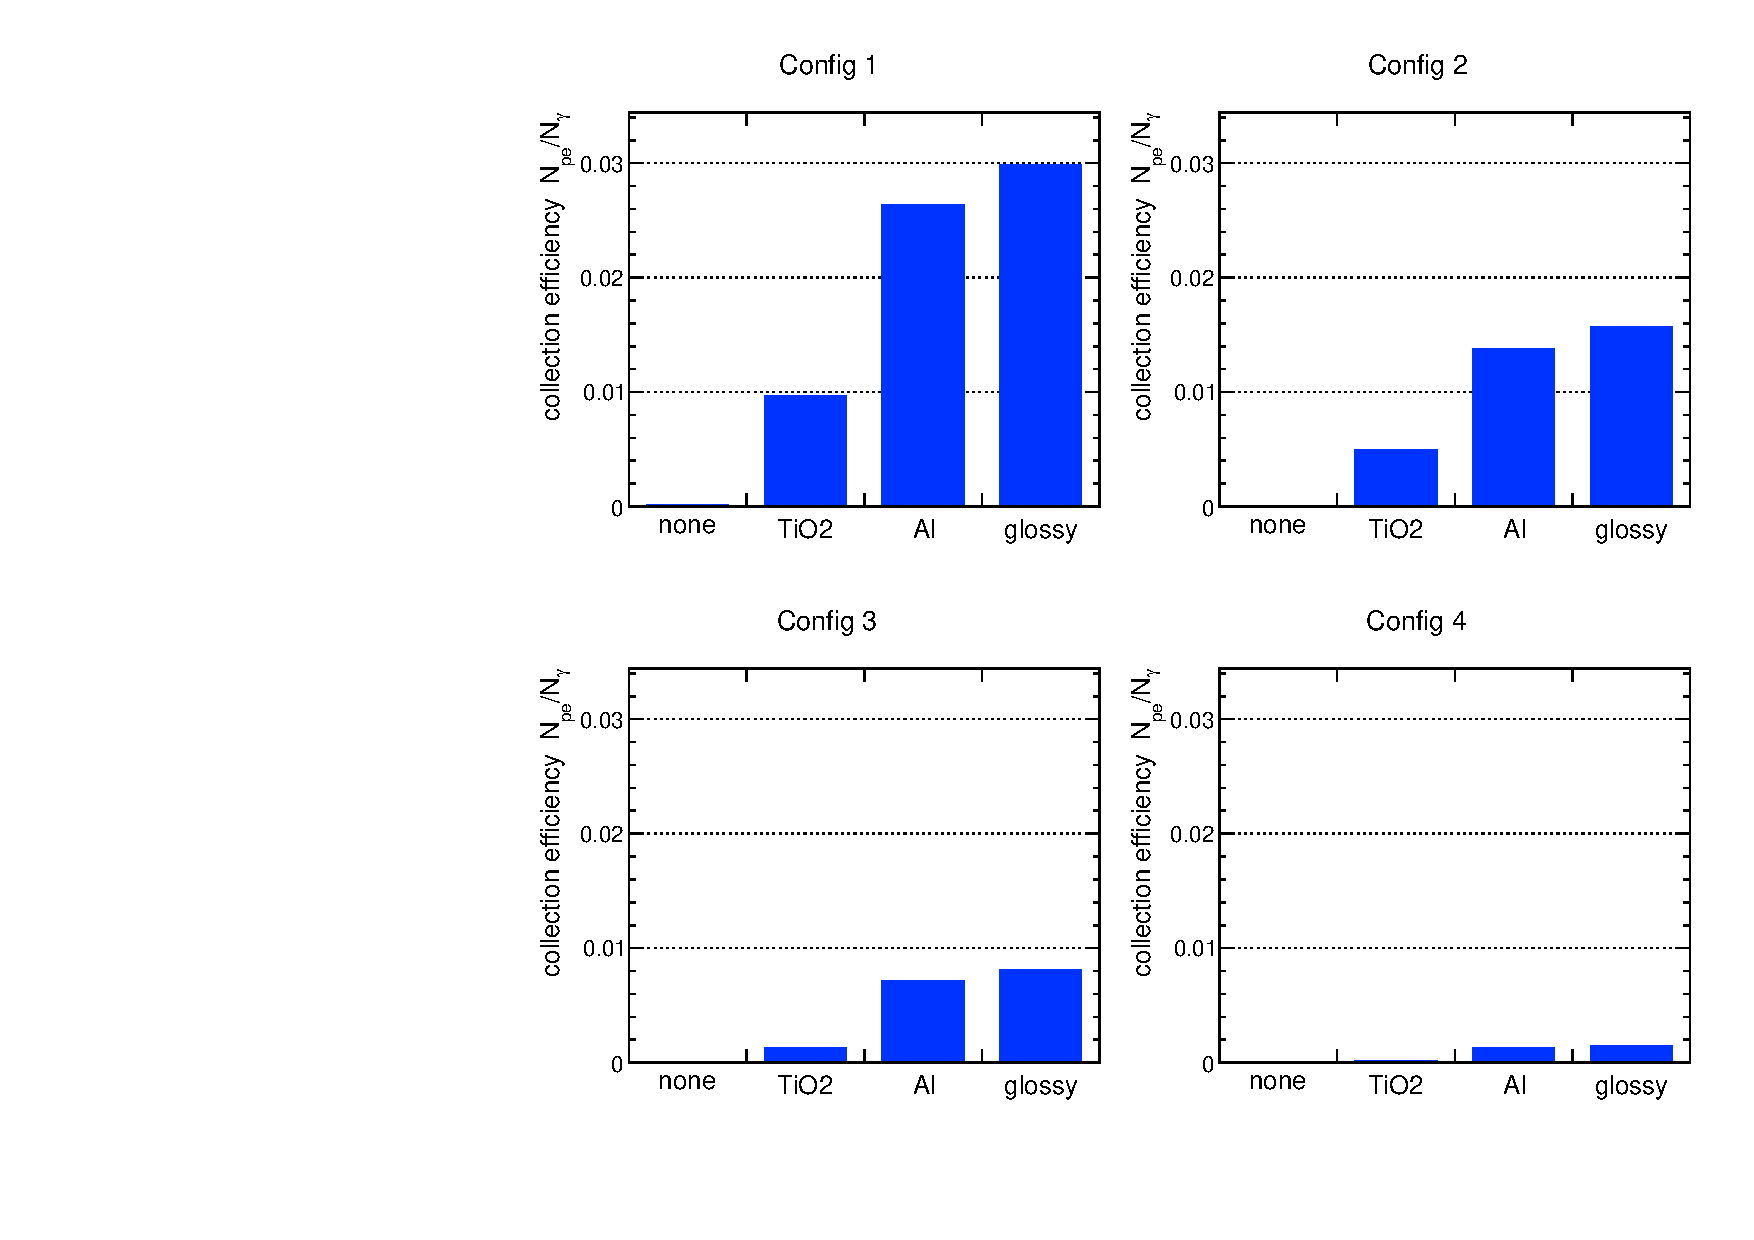
\includegraphics[width=\textwidth]{figures/fig_eff_bars.pdf}
\caption{Overall collection efficiency $\varepsilon = \sum \pe / \sum \ngam$
for the four reflector treatments and four detector layouts. The ordering
$\text{bare} \ll \text{TiO}_2 < \text{Al} \approx \text{glossy}$ is reproduced in
every layout. Error bars assume Poisson counting of photoelectrons.}
\label{fig:bars}
\end{figure}

\begin{table}[H]
\centering
\caption{Overall collection efficiency (all SiPMs, all beam positions pooled).
All beam patches lie fully on the plate.}
\label{tab:eff}
\small
\begin{tabular}{@{}lcccc@{}}
\toprule
Layout & Bare & TiO$_2$ & Al & Glossy \\
\midrule
Config 1 (8 SiPMs) & $1.9\times10^{-4}$ & $9.7\times10^{-3}$ & $2.64\times10^{-2}$ & $2.99\times10^{-2}$ \\
Config 2 (4 SiPMs) & $9.7\times10^{-5}$ & $4.9\times10^{-3}$ & $1.38\times10^{-2}$ & $1.58\times10^{-2}$ \\
Config 3 (2 SiPMs) & $2.3\times10^{-5}$ & $1.30\times10^{-3}$ & $7.17\times10^{-3}$ & $8.16\times10^{-3}$ \\
Config 4 (1 SiPM, WLS) & $6.4\times10^{-6}$ & $2.05\times10^{-4}$ & $1.33\times10^{-3}$ & $1.46\times10^{-3}$ \\
\bottomrule
\end{tabular}
\end{table}

\subsection{Photon yield and photoelectron spectra}

Figure~\ref{fig:yield} shows the per-event optical-photon yield (the
denominator of Eq.~\ref{eq:eff}) for the four reflectors. The mean yield is
essentially independent of the reflector---about \num{19000} photons per event---which is the correct physical behaviour: the reflector changes how
photons are transported, not how many are produced. The small spread reflects
event-to-event variation in the muon path length.

Figure~\ref{fig:detected} shows the corresponding photoelectron spectra. Here the
reflector has a dramatic effect: the bare configuration peaks near zero with a
mean of only \num{3.8}\,\pe/event, whereas glossy paper has a mean of
\num{574}\,\pe/event. The shift from a near-zero-peaked to a broad distribution
is the direct signature of effective light collection.

\begin{figure}[H]
\centering
\begin{subfigure}{0.49\textwidth}
  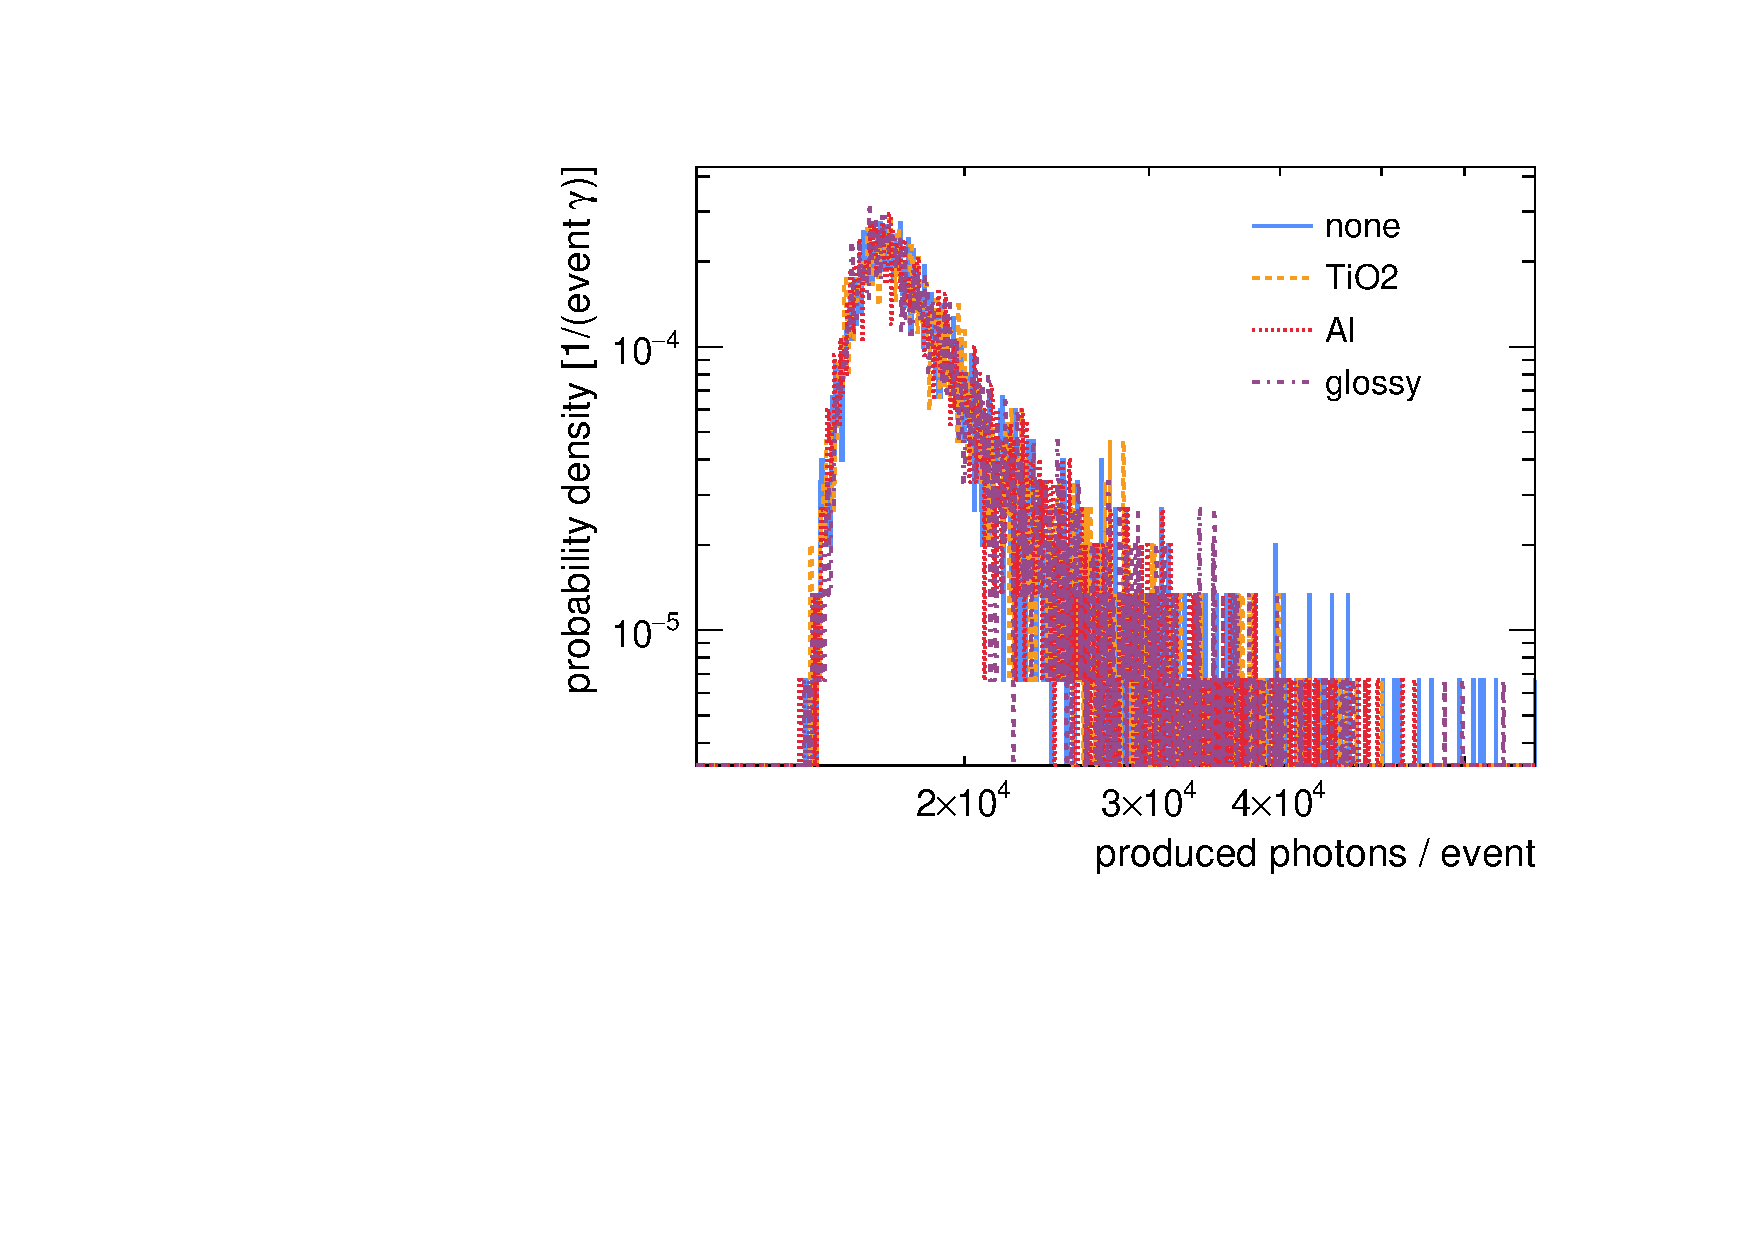
\includegraphics[width=\textwidth]{figures/fig_yield.pdf}
  \caption{Yield (produced photons/event).}
  \label{fig:yield}
\end{subfigure}\hfill
\begin{subfigure}{0.49\textwidth}
  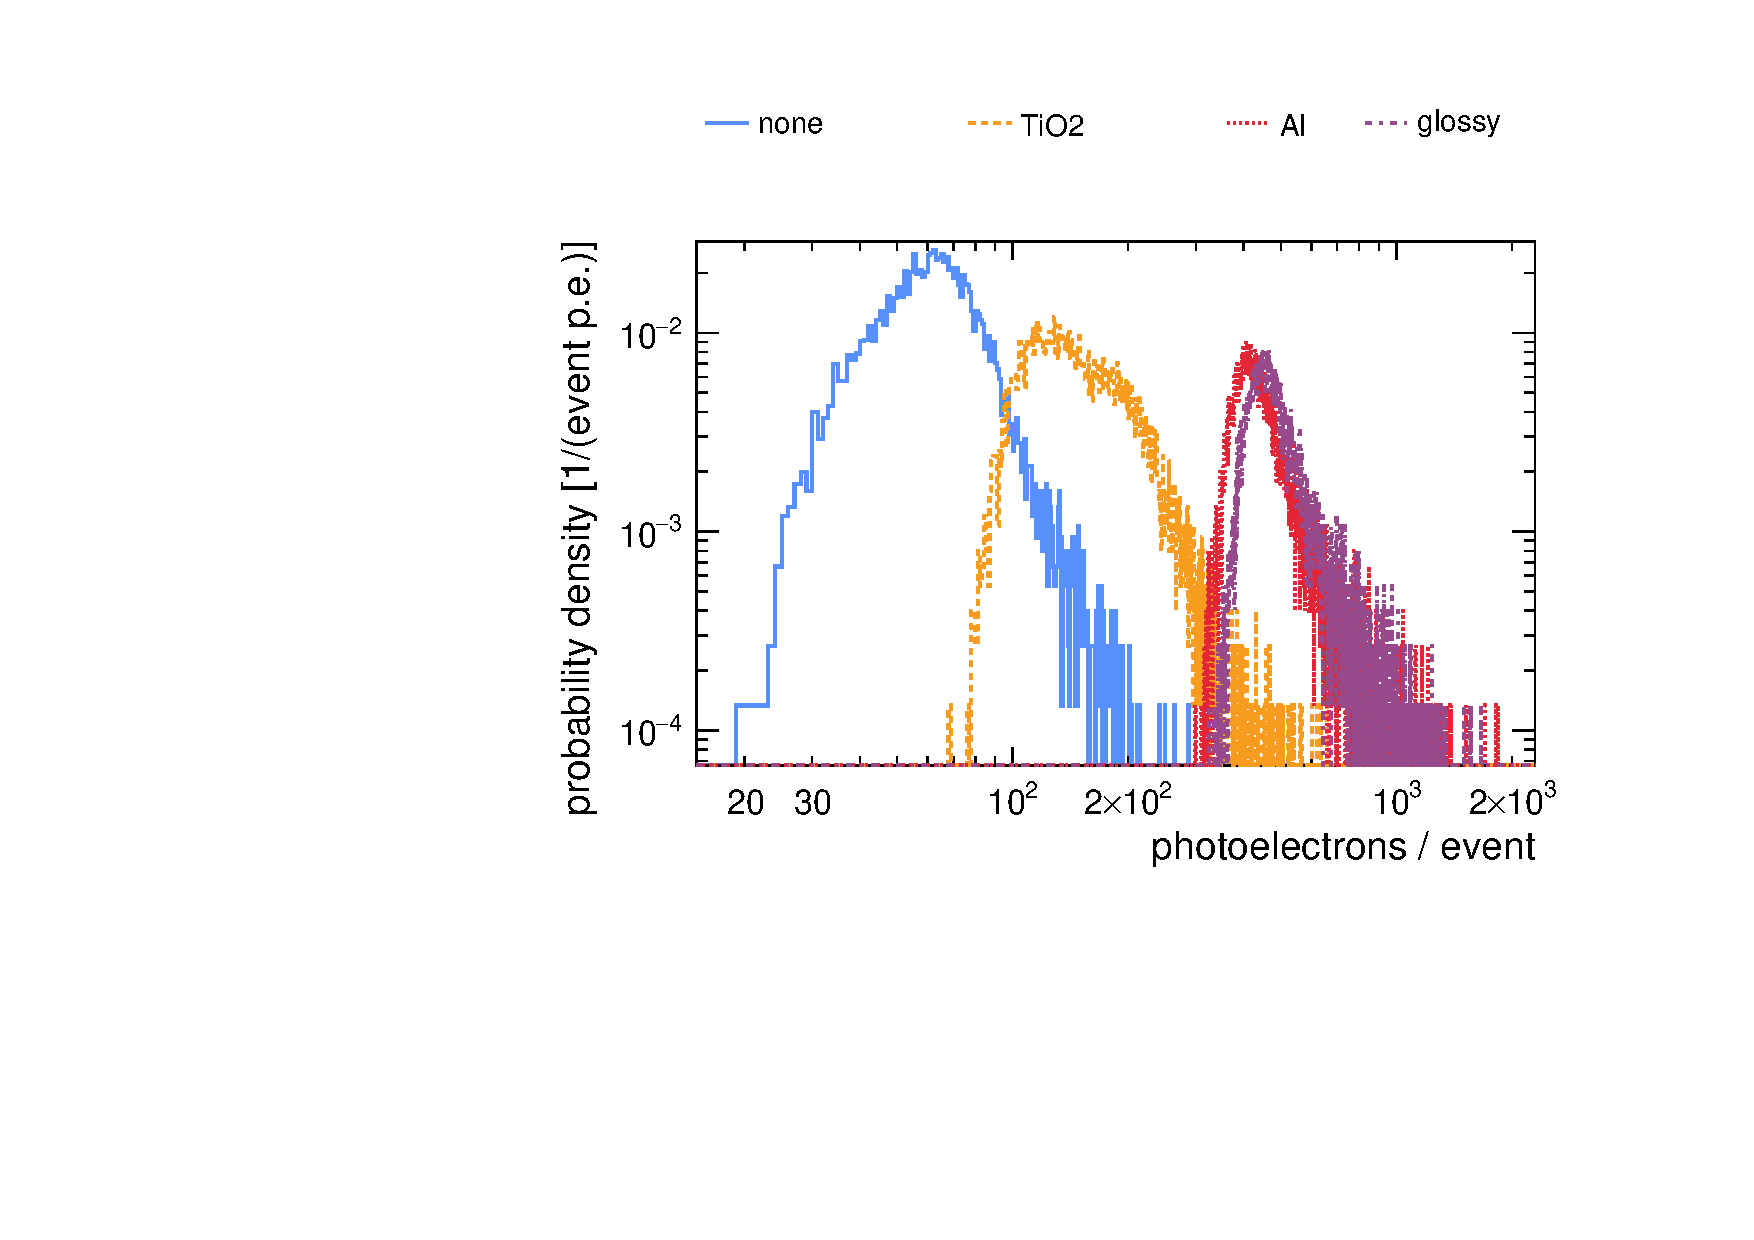
\includegraphics[width=\textwidth]{figures/fig_detected.pdf}
  \caption{Photoelectrons/event.}
  \label{fig:detected}
\end{subfigure}
\caption{Per-event distributions for config~1, plotted as a probability density
(unit area, \SI{1}{\per event} per unit of the abscissa) with logarithmic $x$- and
$y$-axes. The production yield (left) is reflector-independent, as it must be; the
detected photoelectron count (right) depends strongly on the wrapper. The log
$y$-axis is needed because the four curves have the same event count but very
different widths: the concentrated bare peak and the broad reflective
distributions cannot both be resolved on a linear scale.}
\label{fig:spectra}
\end{figure}

The efficiency scale is set by the SiPM PDE and the coupling: of order
\num{19000} photons are produced and the best wrapper delivers
$\approx 574$ photoelectrons, i.e.\ $\approx 3\%$. Given a PDE of
$\sim\!0.4$ and the geometric acceptance of a side-mounted sensor, this is
consistent.

\subsection{Wavelength of detected photons}

Figure~\ref{fig:wavelength} shows the wavelength distribution of detected
photoelectrons, weighted by their count, for the four reflectors. The
distribution peaks near \SI{460}{\nano\meter} for the reflective wrappers
(measured mean $459.5 \pm 4.7\,\mathrm{nm}$ for Al, config~1), i.e.\ slightly
red-shifted with respect to the \SI{425}{\nano\meter} emission peak. This is the
expected consequence of self-absorption: the shorter-wavelength part of the
emission overlaps the absorption band and is attenuated over the multi-bounce
path, so the surviving and detected spectrum is red-shifted. The bare
configuration has too few detected photons for a meaningful spectrum.

\begin{figure}[H]
\centering
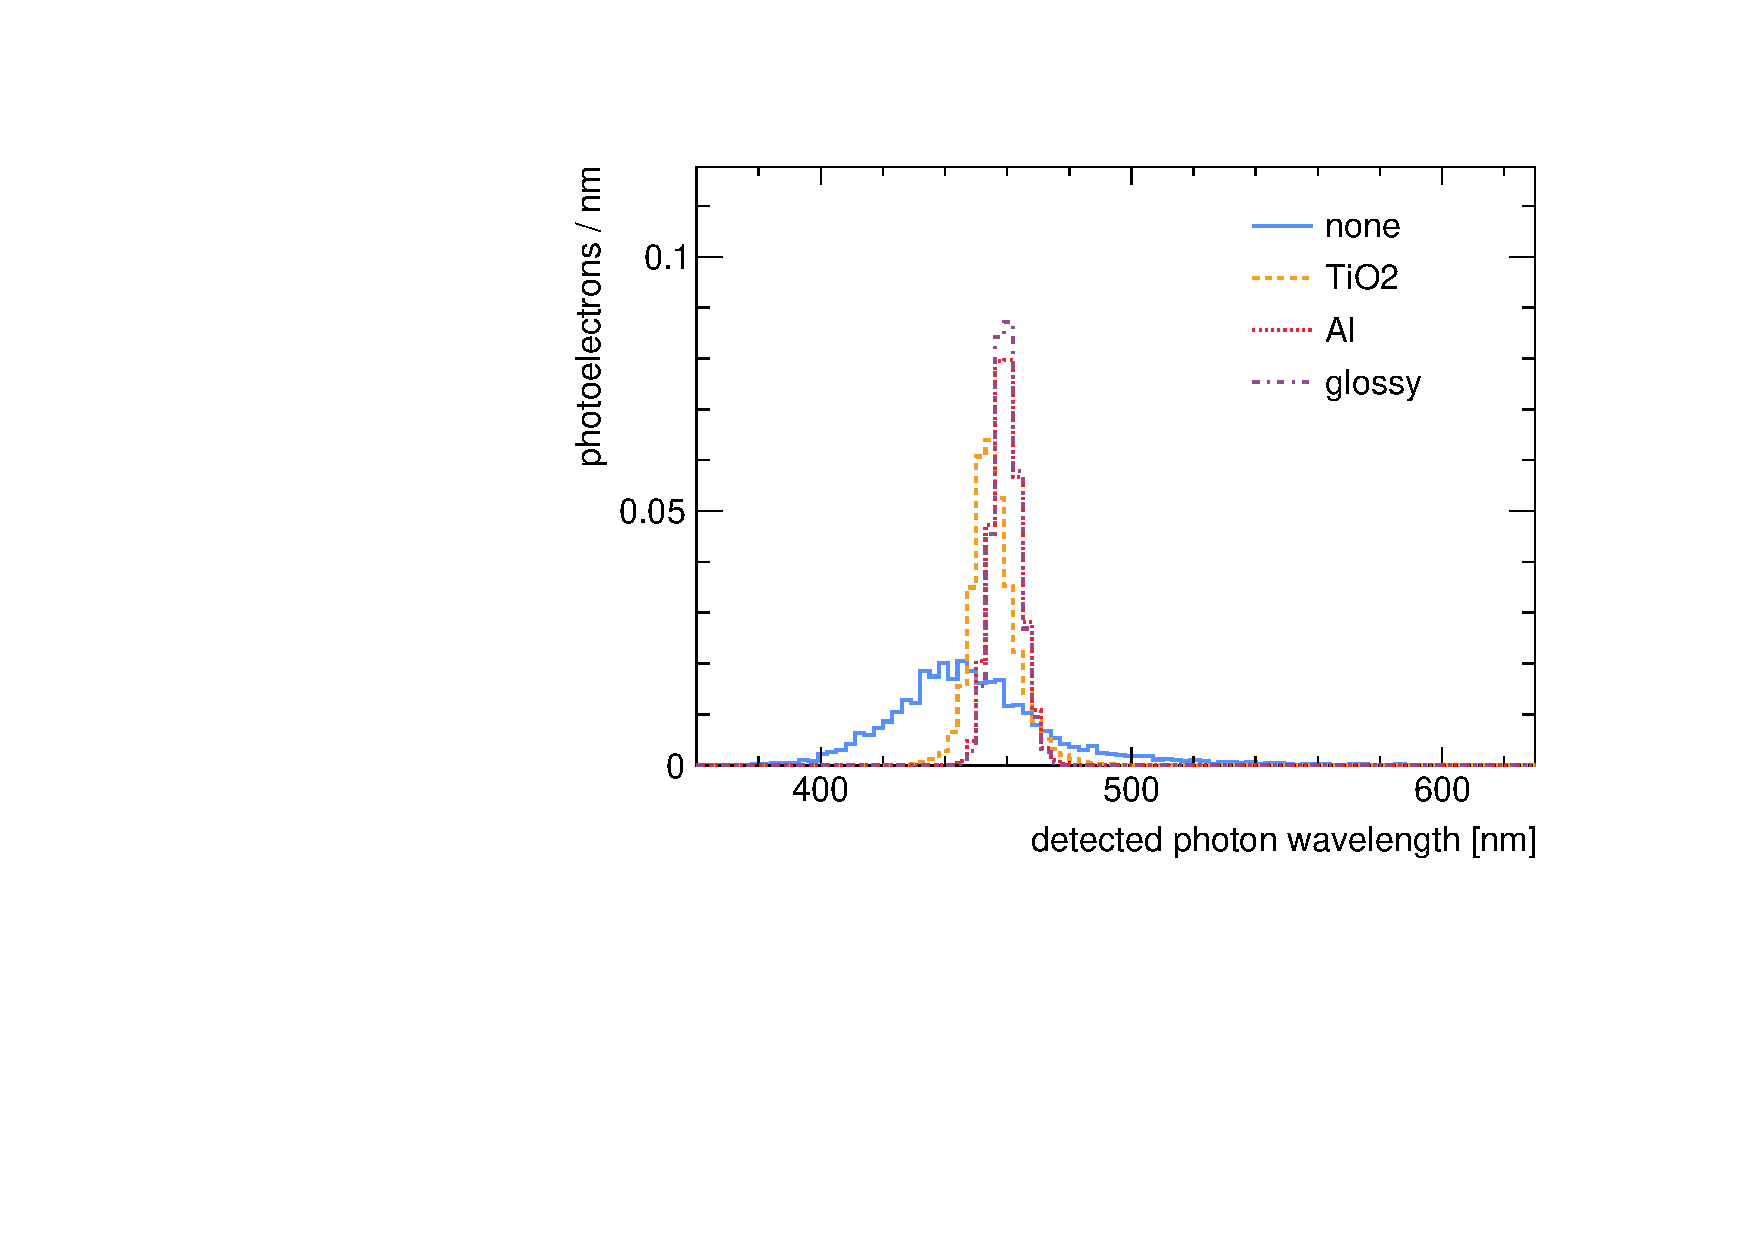
\includegraphics[width=0.62\textwidth]{figures/fig_wavelength.pdf}
\caption{Wavelength distribution of detected photoelectrons (config~1), weighted
by detected count. The reflective wrappers give a distribution peaking near
\SI{460}{\nano\meter}, red-shifted from the \SI{425}{\nano\meter} emission peak
by self-absorption over the multi-bounce path.}
\label{fig:wavelength}
\end{figure}

Figure~\ref{fig:wavelengthcfg} compares the detected-photon spectrum of the four
configurations for each wrapper. Configurations~1--3, in which the SiPMs view the
tile directly, all detect the same blue scintillation spectrum: the
\emph{mean} wavelength is essentially independent of the number of sensors,
moving only from \SI{459.5}{\nano\meter} (glossy, config~1) to
\SI{460.3}{\nano\meter} (config~3), the small increase reflecting the slightly
longer collection path of the single-sided layouts. Config~4 is qualitatively
different: the WLS fibres absorb the blue light and re-emit it at their own
emission band, so the detected spectrum is shifted to
\SI{480.6}{\nano\meter} (glossy) --- a green-shift of some
\SI{20}{\nano\meter}. The same shift appears for every wrapper, including the
bare tile (which, with its very small photon count, is statistically noisy),
confirming that it originates in the fibre wavelength shifter rather than in the
wrapper.

\begin{figure}[H]
\centering
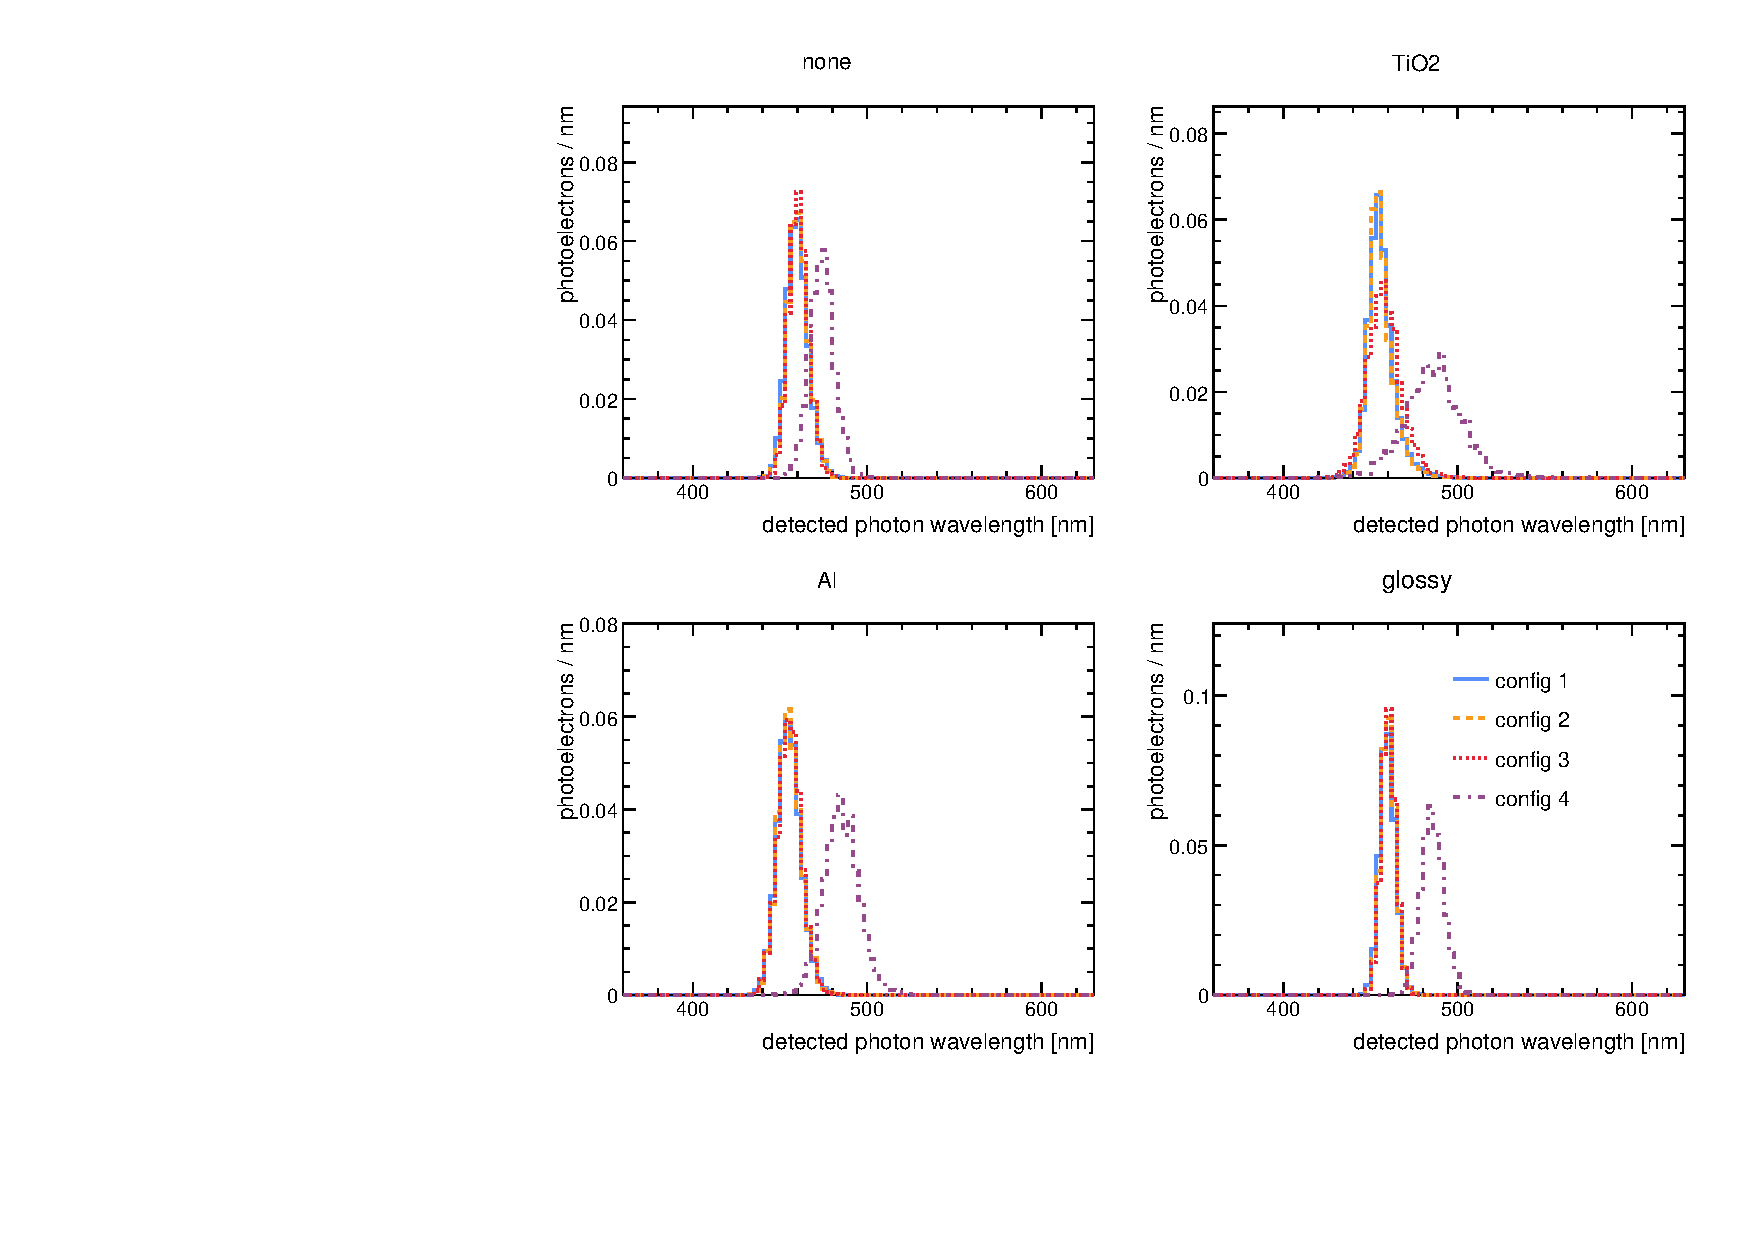
\includegraphics[width=0.9\textwidth]{figures/fig_wavelength_cfg.pdf}
\caption{Detected-photon wavelength distribution, weighted by photoelectron
count, for each wrapper (panel) and each configuration (curves), using the
pooled data of the three irradiation positions. Configurations~1--3 follow the
\SI{460}{\nano\meter} blue scintillation spectrum regardless of sensor count,
whereas the WLS-fibre readout of config~4 is green-shifted to
$\approx \SI{480}{\nano\meter}$ by the Y-11(200) emission band.}
\label{fig:wavelengthcfg}
\end{figure}

\subsection{Spatial and directional dependence}

The matrix scan separates the three \SI{50}{\milli\meter}$\times$\SI{50}{\milli\meter}
patches (centre, edge, corner) precisely so that the response can be resolved by
position. The tempting single-coordinate summary is the distance $r$ of the patch
from the plate centre, but $r$ is blind to azimuth, and the shortcoming is
decisive here: configs~3 and~4 instrument a \emph{single} face, so the collection
depends on the \emph{direction} from which the plate is irradiated, not merely on
the distance. All three patches also lie on the half of the plate opposite the
instrumented face of the single-sided layouts, so their distances are not even
monotonic in the proximity to a sensor. We therefore keep the three patches
separate and compare them directly.

Figure~\ref{fig:poslayouts} groups the three patches by layout (one panel per
config, four reflector curves) and Fig.~\ref{fig:posrefl} groups them by
reflector (one panel per wrapper, four layout curves). Because every patch lies
fully on the plate and all three have equal area, the produced-photon
denominators are equal and the three points within each curve are directly
comparable. The curves are plotted on a logarithmic $y$-axis, so the weakly
collecting bare plate is resolved alongside the reflective wrappers.

The conspicuous feature is that the reflective wrappers \emph{homogenise} the
response: for Al and glossy paper the efficiency varies by at most
\SIrange{1}{9}{\percent} across the three patches in every layout
(Fig.~\ref{fig:uniformity} and Table~\ref{tab:contrast}), i.e.\ an
edge- or corner-irradiated plate collects almost exactly as much light as a
centre-irradiated one. To quantify this we define the \emph{position contrast}
\begin{equation}
  \kappa \equiv \frac{\varepsilon_{\max}}{\varepsilon_{\min}},
  \label{eq:contrast}
\end{equation}
the ratio of the largest to the smallest of the three patch-averaged collection
efficiencies $\varepsilon$ (Eq.~\ref{eq:eff}), so that $\kappa=1$ denotes a
perfectly uniform response and $\kappa-1$ the fractional spread. The diffuse
TiO$_2$ paint is markedly less uniform (a
factor $\approx\!1.7$--$1.9$), and the bare plate records by far the strongest
position dependence (up to a factor \num{8} for config~4, whose single readout
amplifies any asymmetry). This is the expected behaviour of a closed reflecting
cavity: after the first few bounces the light distribution no longer remembers
where the muon crossed the plate, so the sensor coverage, and not the irradiation
point, sets the collection. A single-sided layout is the extreme test of this
argument, and even there the mirror wrappers keep the position contrast below
\SI{10}{\percent}.

\begin{figure}[H]
\centering
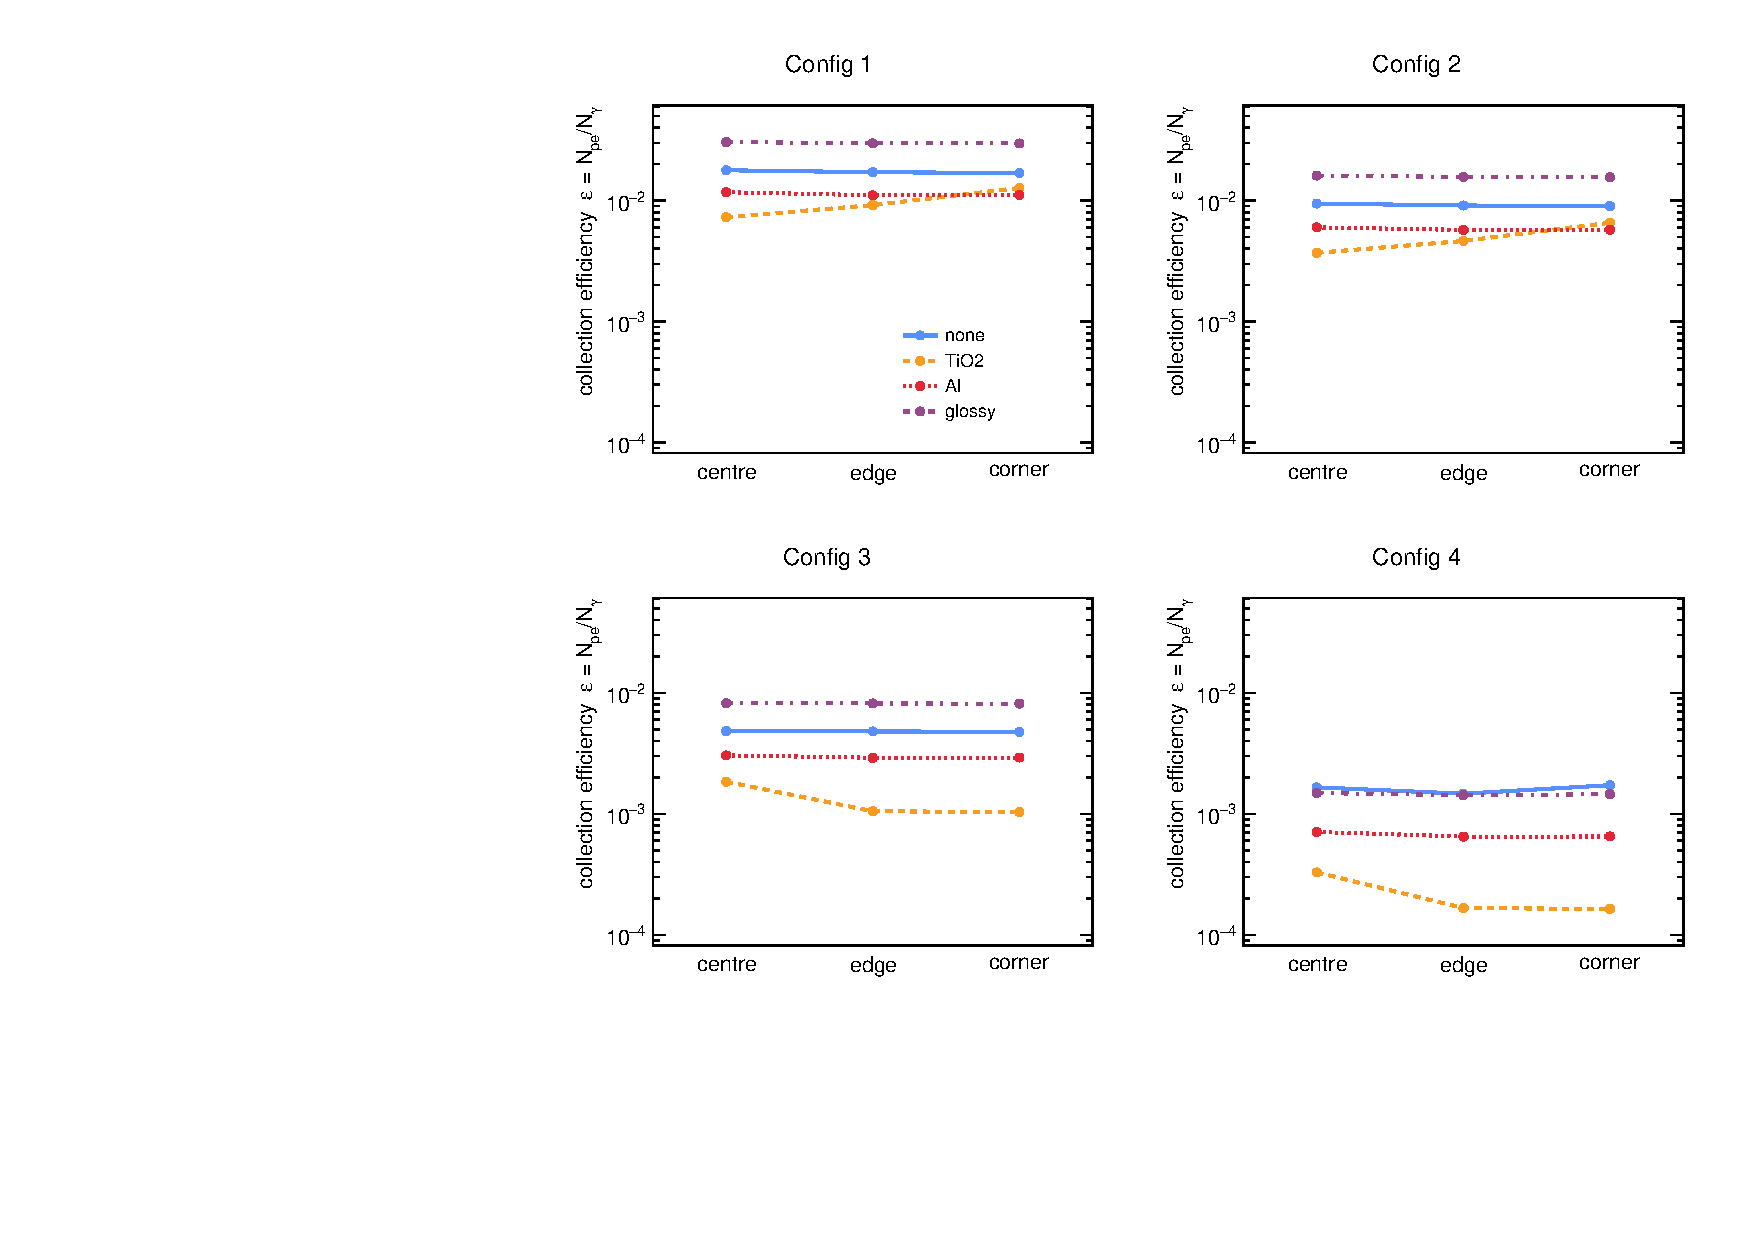
\includegraphics[width=\textwidth]{figures/fig_pos_layouts.pdf}
\caption{Collection efficiency at the three irradiation patches (centre, edge,
corner), one panel per detector layout, with the four reflector curves
(logarithmic $y$-axis). All three patches have equal area and lie fully on the
plate, so the points are directly comparable. The reflective wrappers are nearly
flat across the three patches in every layout; the bare plate is both weakest and
most position-dependent.}
\label{fig:poslayouts}
\end{figure}

\begin{figure}[H]
\centering
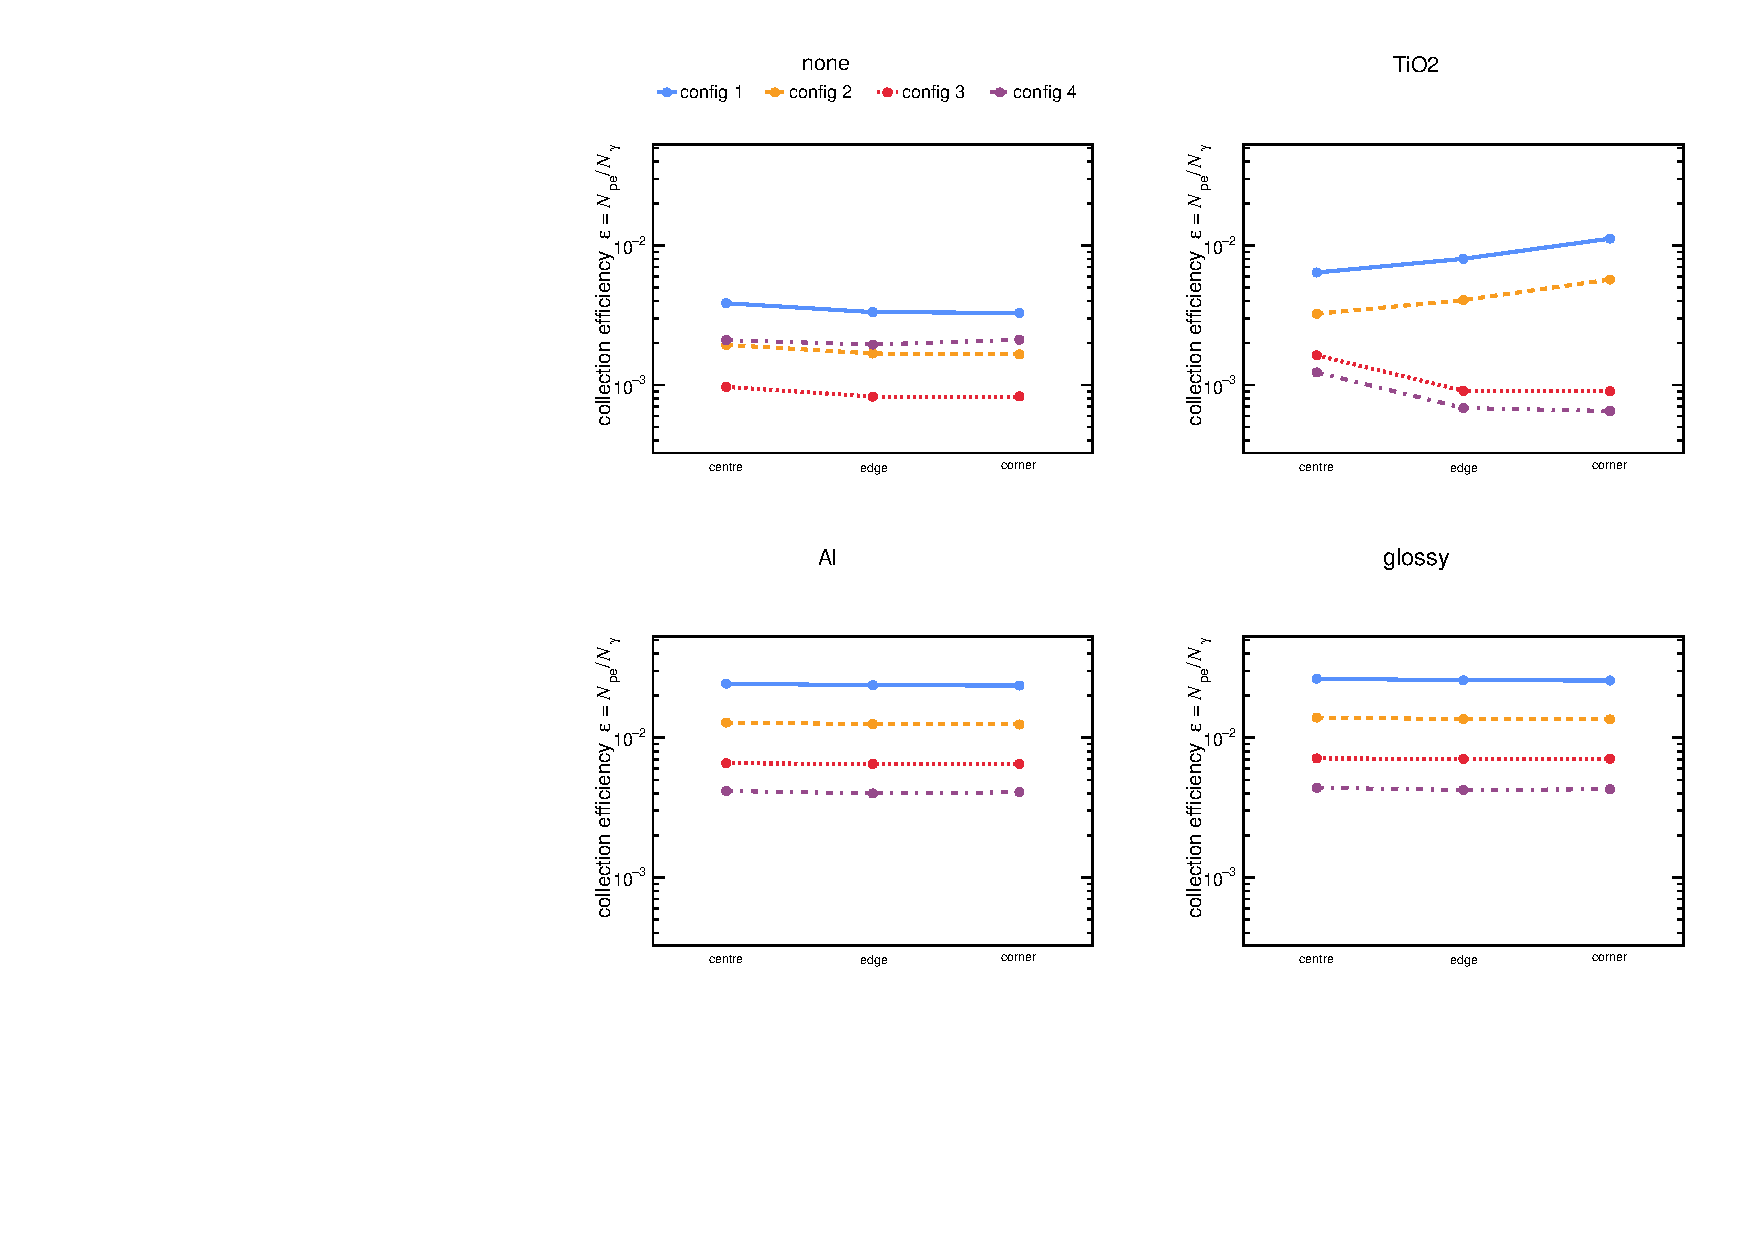
\includegraphics[width=\textwidth]{figures/fig_pos_refl.pdf}
\caption{The same data grouped by reflector (one panel per wrapper), with the
four layouts as curves. Configs~1 and~2 (sensors on every face) are the most
uniform; the single-sided layouts (3 and~4) drop toward the edge and corner
patches, which sit on the far side of the plate from their sensors.}
\label{fig:posrefl}
\end{figure}

\begin{figure}[H]
\centering
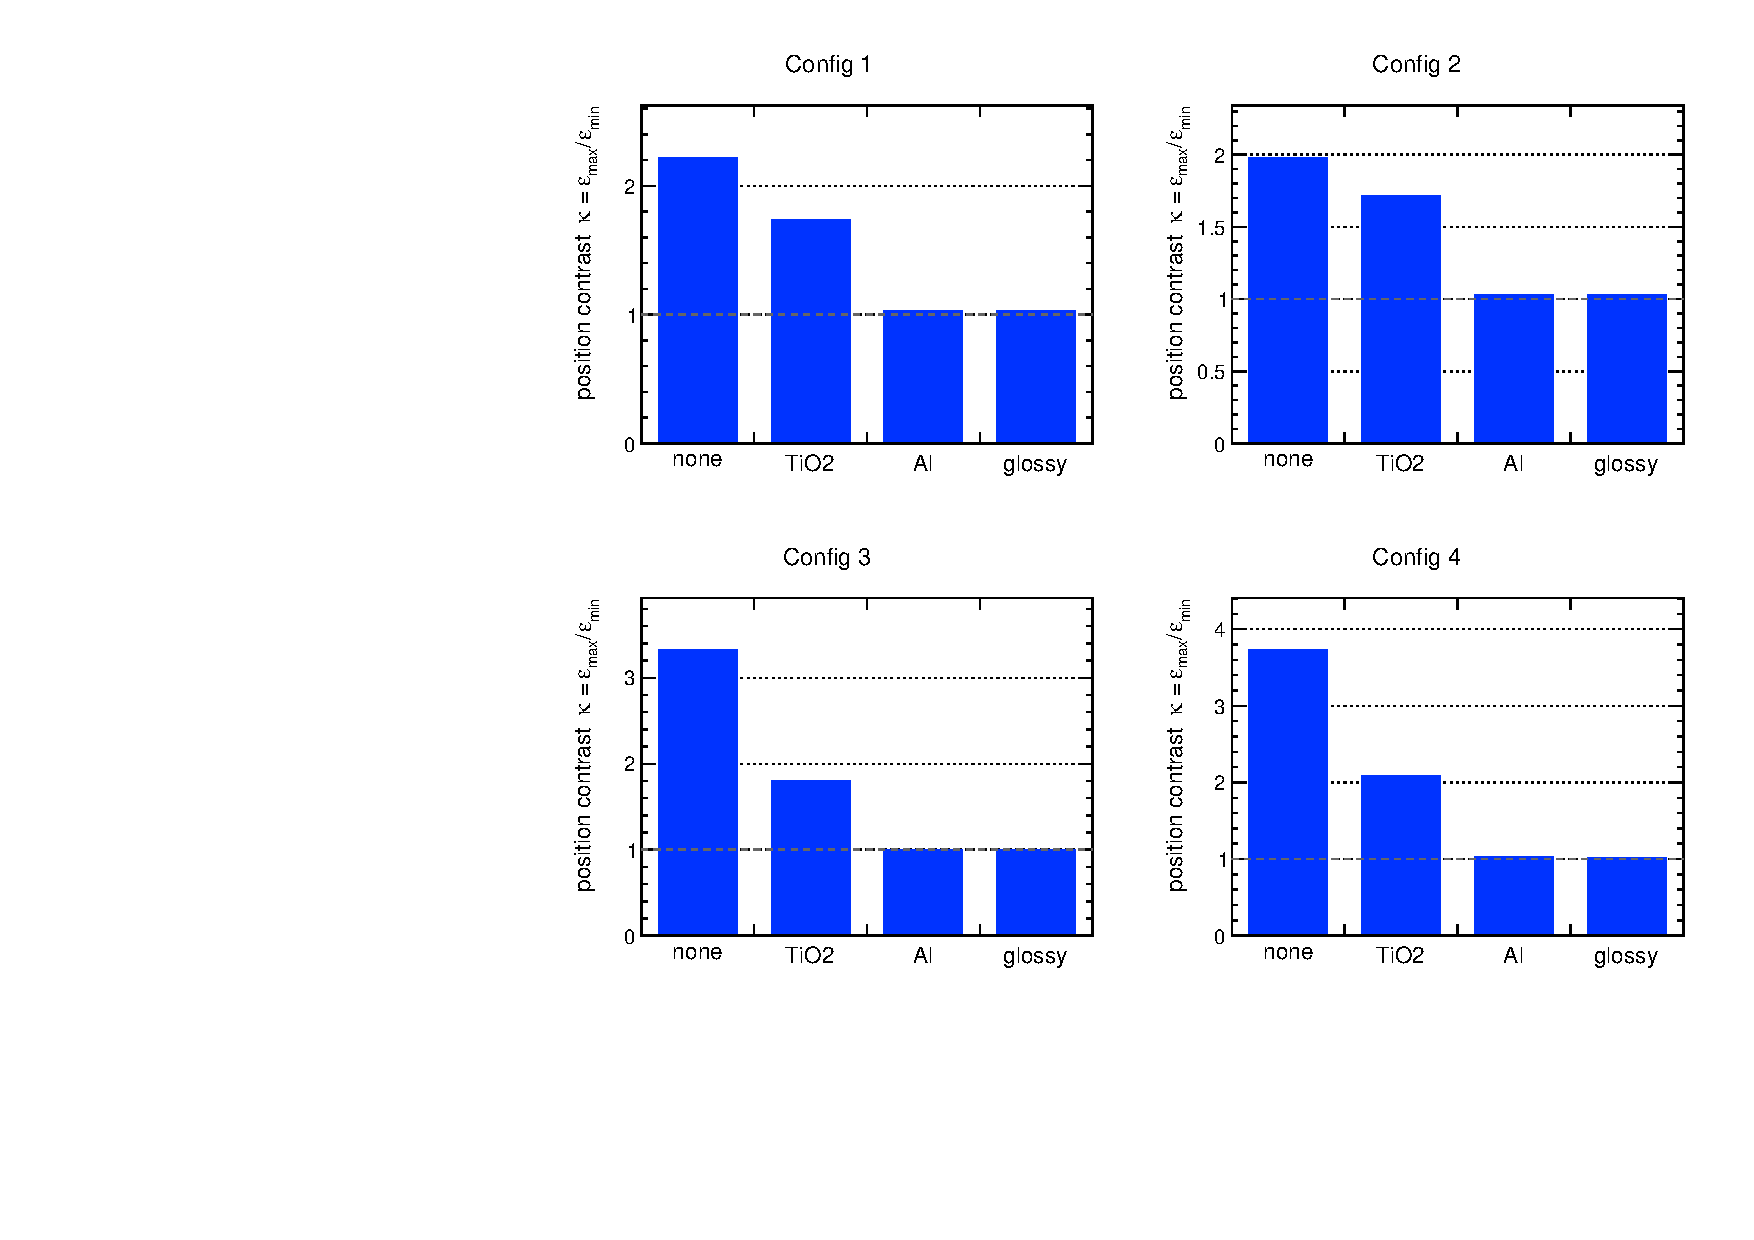
\includegraphics[width=\textwidth]{figures/fig_uniformity.pdf}
\caption{Position contrast $\kappa = \varepsilon_{\max}/\varepsilon_{\min}$
(Eq.~\ref{eq:contrast}) over the three
irradiation patches, one panel per layout, four reflector bars (dashed line:
$\kappa=1$). The mirror-like wrappers hold the
contrast within \SI{9}{\percent} in every layout, whereas diffuse TiO$_2$ and
especially the bare plate are strongly position-dependent.}
\label{fig:uniformity}
\end{figure}

\begin{table}[H]
\centering
\caption{Position contrast $\kappa = \varepsilon_{\max}/\varepsilon_{\min}$
(Eq.~\ref{eq:contrast}) across the
three irradiation patches (centre, edge, corner). A value of~1 means the layout
collects the same fraction of light wherever the muon crosses the plate.}
\label{tab:contrast}
\small
\begin{tabular}{@{}lcccc@{}}
\toprule
Reflector & Config 1 & Config 2 & Config 3 & Config 4 \\
\midrule
Bare   & 2.15 & 2.03 & 3.56 & 8.22 \\
TiO$_2$& 1.74 & 1.75 & 1.77 & 1.93 \\
Al     & 1.04 & 1.03 & 1.01 & 1.09 \\
Glossy & 1.03 & 1.03 & 1.00 & 1.09 \\
\bottomrule
\end{tabular}
\end{table}

Figure~\ref{fig:sharing} resolves the directional response most directly. For
config~1 (the layout with the most sensors) it shows the \emph{share} of the
collected light seen by each of the eight sensors, in one panel per reflector,
with the three irradiation patches as grouped bars (dashed line: the uniform
expectation of $1/8$). The difference between the
wrappers is stark. For the \emph{bare} plate the light barely mixes: at the
corner patch the two sensors nearest the beam ($\mathrm{B2}$, $\mathrm{R1}$)
together collect \SI{91}{\percent} of all photoelectrons, i.e.\ some \num{3.6}
times the uniform share each, while the remaining six share only
\SI{9}{\percent} and two of them ($\mathrm{B1}$, $\mathrm{R2}$) record nothing
at all. A diffuse or mirror wrapper erases this
structure: for glossy paper the same two nearest sensors reach only about
\num{1.1} times the uniform share. The total efficiency is nearly the same for all
three patches (Table~\ref{tab:contrast}), so the cavity keeps the \emph{amount}
of collected light constant while completely rearranging its spatial division.
A radius-only summary averages these distinct per-sensor patterns into a single
number and hides precisely this information.

\begin{figure}[H]
\centering
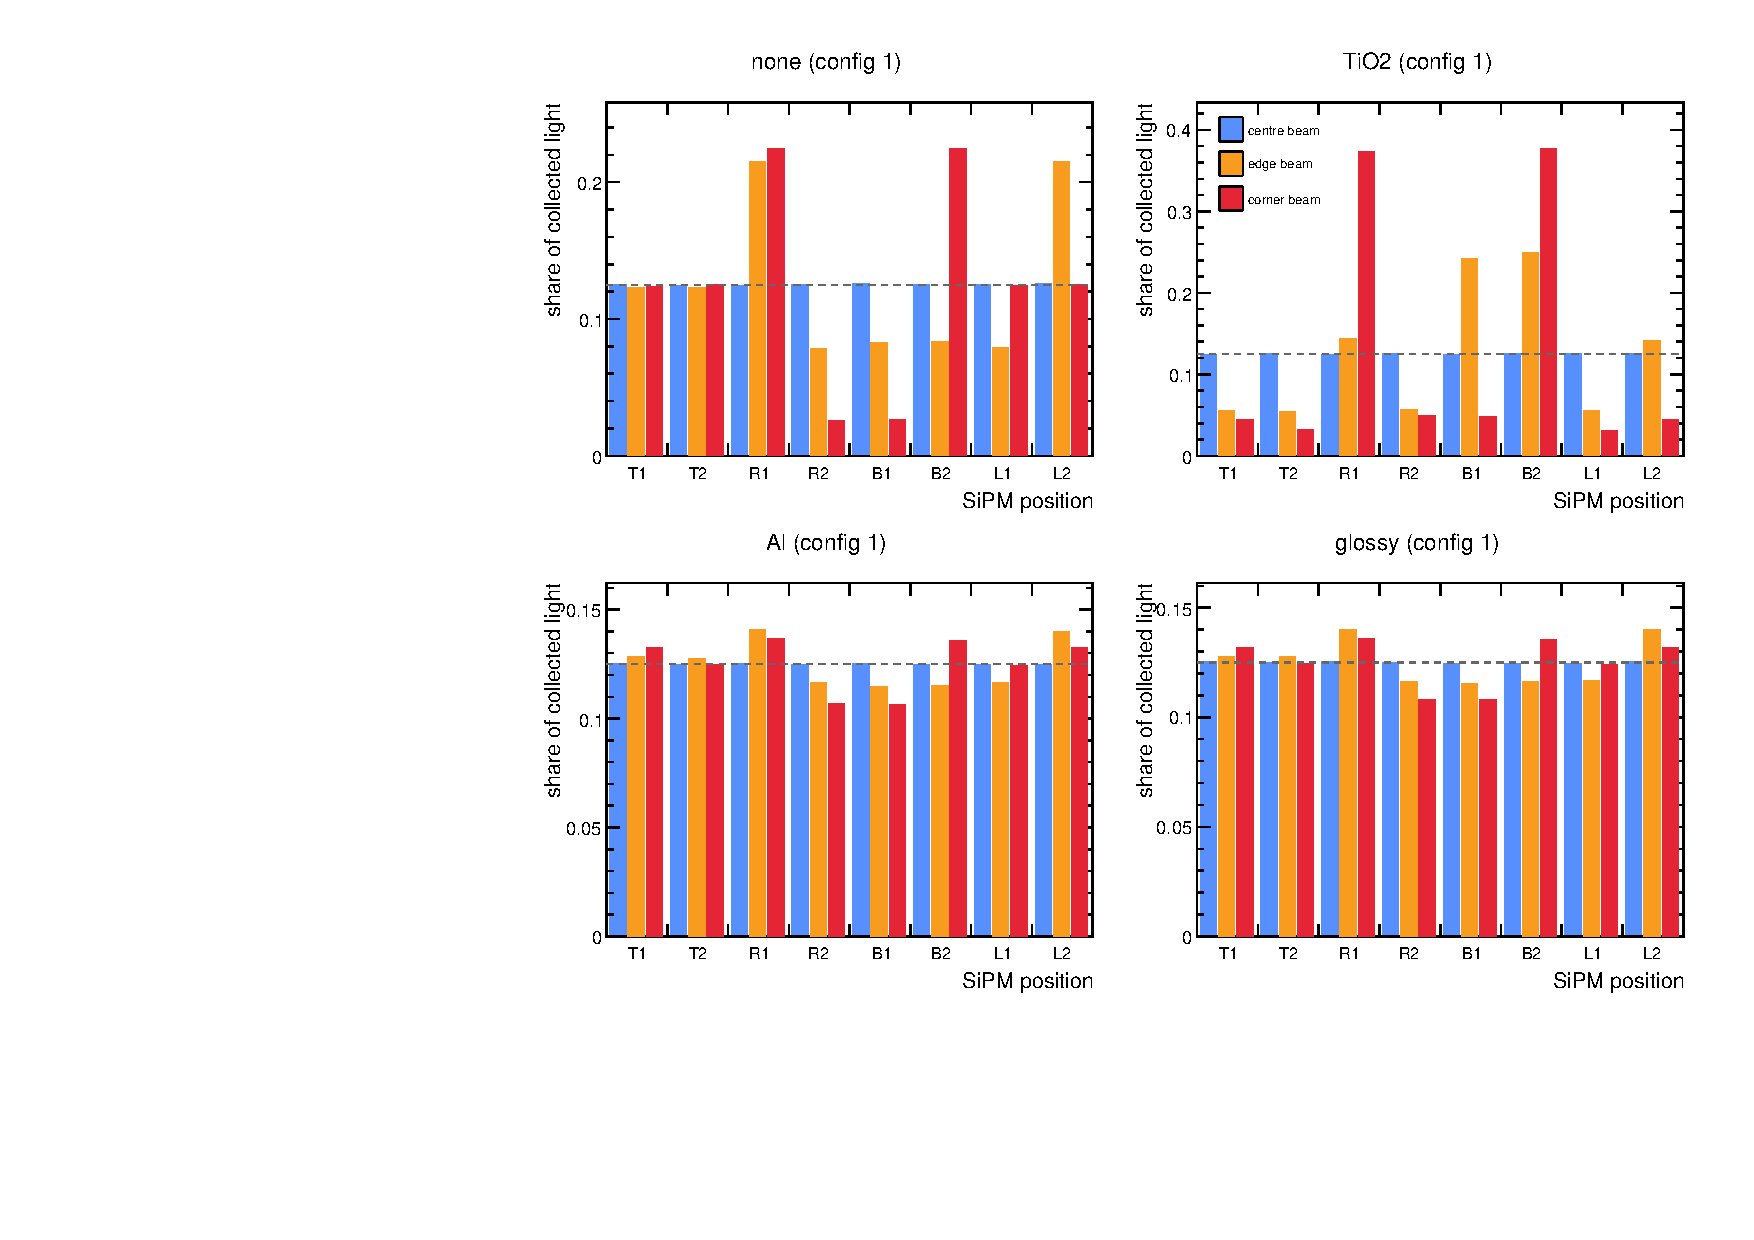
\includegraphics[width=\textwidth]{figures/fig_sipm_sharing.pdf}
\caption{Direction-aware light sharing, config~1, one panel per reflector. Each
group of bars is one sensor (x axis) and the three colours are the irradiation
patches (blue: centre, orange: edge, red: corner); the height is that sensor's
share of the light collected at that patch, and the dashed line marks the
uniform expectation $1/8$. For the bare plate the light stays concentrated on
the two sensors nearest the beam, whereas the reflective wrappers spread it
almost uniformly over all eight.}
\label{fig:sharing}
\end{figure}

\subsection{Position-resolved efficiency maps}

Figures~\ref{fig:grid1}--\ref{fig:grid4} show the two-dimensional collection
efficiency as a function of the muon entry point $(x,y)$, one panel per
reflector, for the four configurations. Each map is the ratio of collected
photoelectrons to produced photons in $5 \times \SI{5}{\milli\meter}$ cells
(Eq.~\ref{eq:eff}, evaluated bin-by-bin). The black squares mark the SiPM
positions for that configuration (same convention as Fig.~\ref{fig:layouts}).
Because the matrix scan only
irradiates the three \SI{50}{\milli\meter}$\times$\SI{50}{\milli\meter} patches,
only those regions are populated; the maps therefore show the internal structure
of each of the three fields. Within a patch the reflective wrappers are almost
featureless---consistent with the near-uniform integrated response found
above---while the bare plate and, to a lesser degree, the TiO$_2$ coating show a
clear gradient across the field, brightest on the side nearest the sensors.

Table~\ref{tab:positions} lists the absolute centre/edge/corner efficiencies for
config~1; the position- and direction-resolved comparison across all four layouts
is the subject of the preceding subsection
(Figs.~\ref{fig:poslayouts}--\ref{fig:sharing}), and the TiO$_2$ corner excess it
reveals is discussed in Sec.~\ref{sec:caveats}.

\begin{figure}[H]
\centering
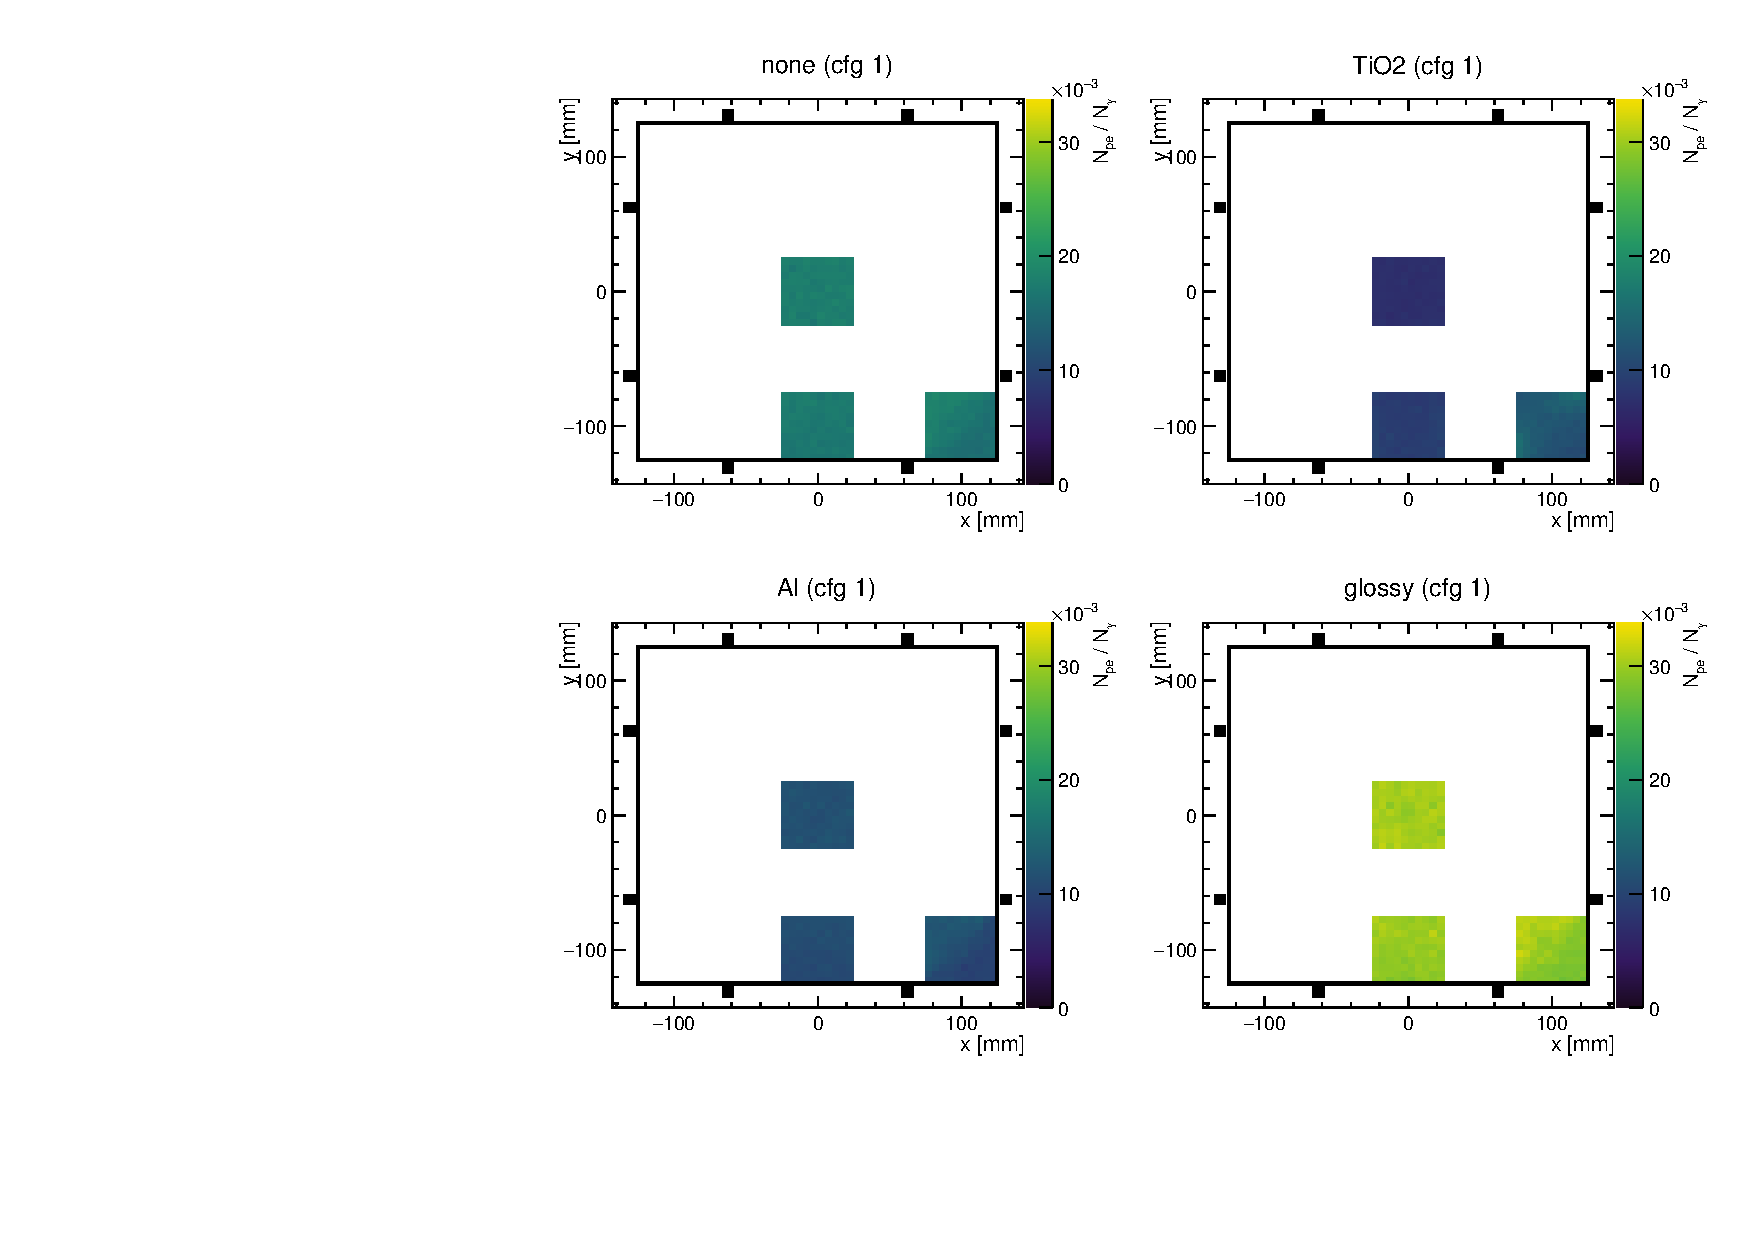
\includegraphics[width=\textwidth]{figures/efficiency_grid_cfg1_all.pdf}
\caption{Collection efficiency map, config~1 (8 SiPMs), one panel per reflector
(bare, TiO$_2$, Al, glossy). Bins are $5 \times \SI{5}{\milli\meter}$; black
squares mark the SiPM positions (two per edge).}
\label{fig:grid1}
\end{figure}

\begin{figure}[H]
\centering
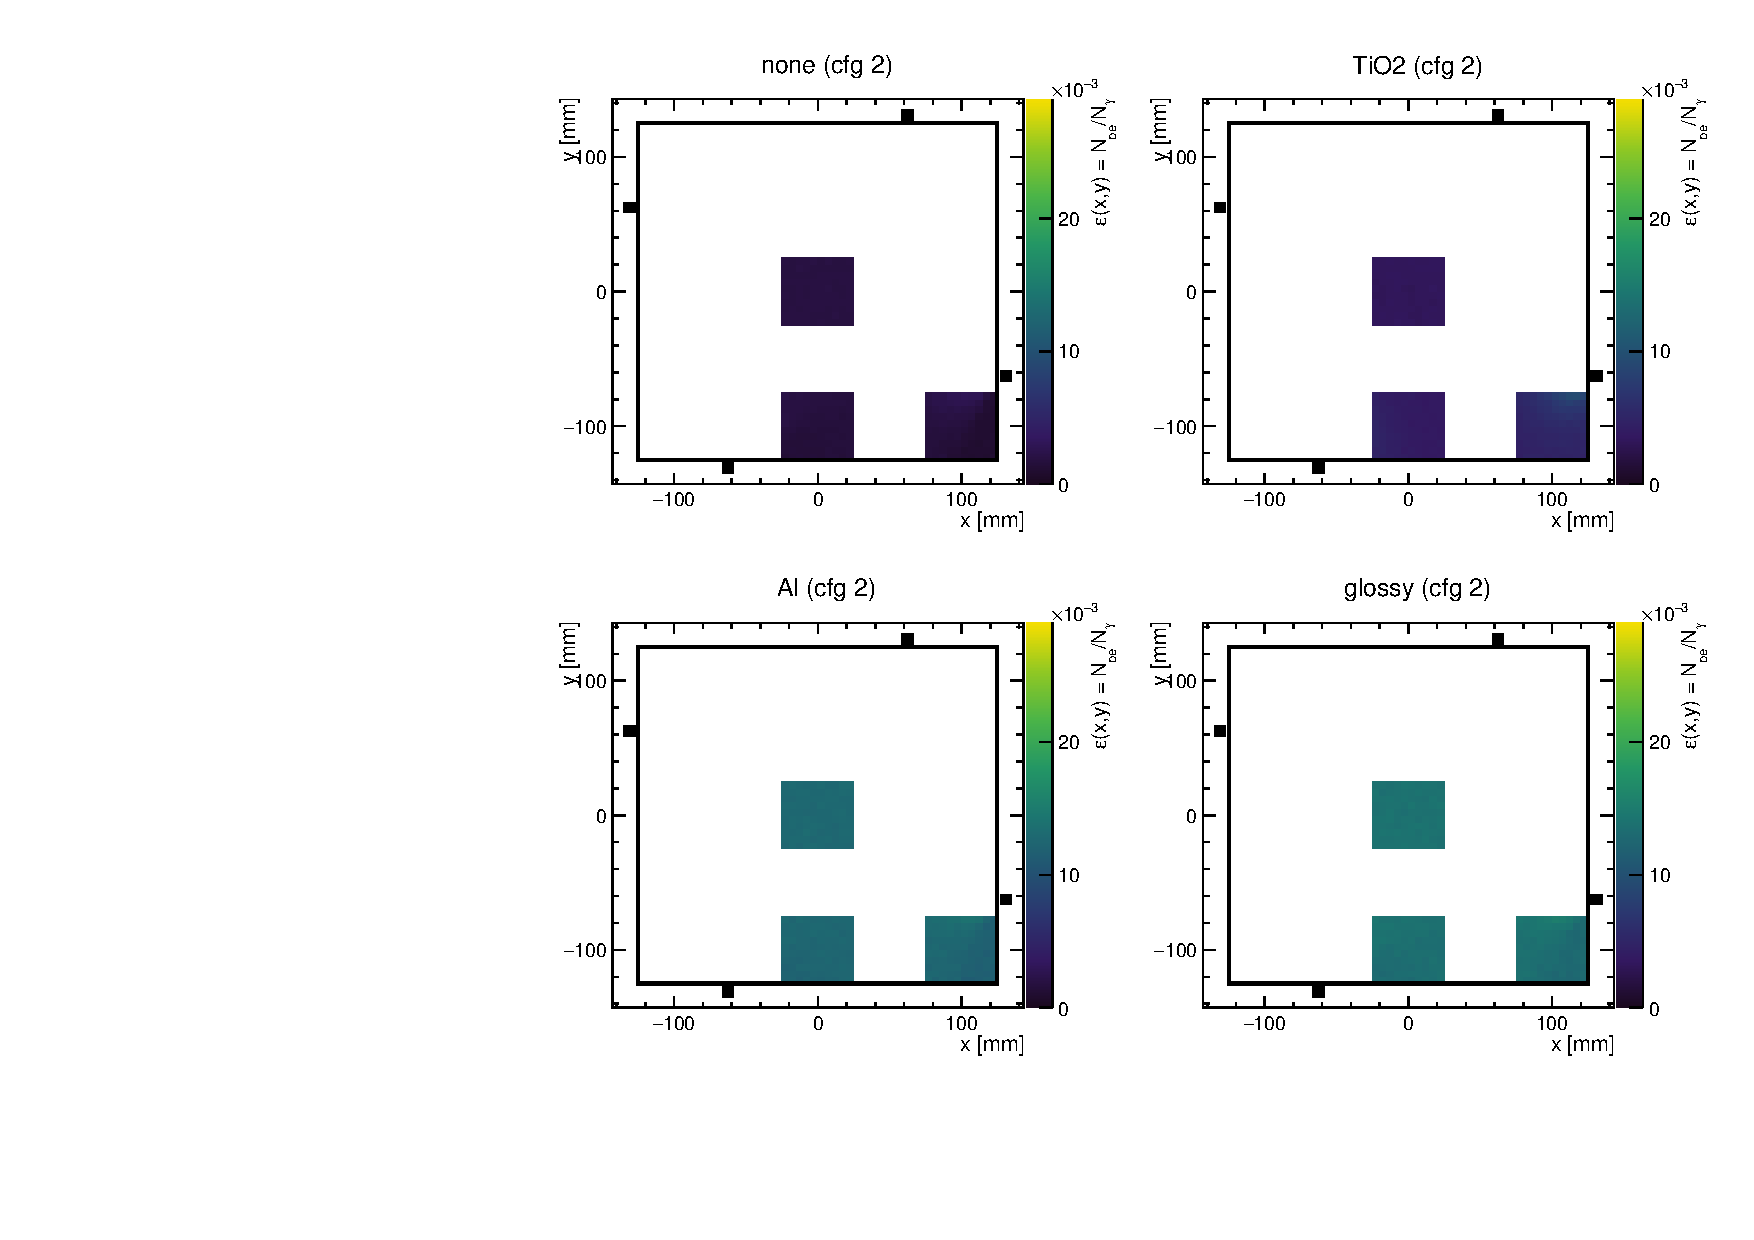
\includegraphics[width=\textwidth]{figures/efficiency_grid_cfg2_all.pdf}
\caption{Collection efficiency map, config~2 (4 SiPMs, one per side). Black
squares mark the SiPM positions.}
\label{fig:grid2}
\end{figure}

\begin{figure}[H]
\centering
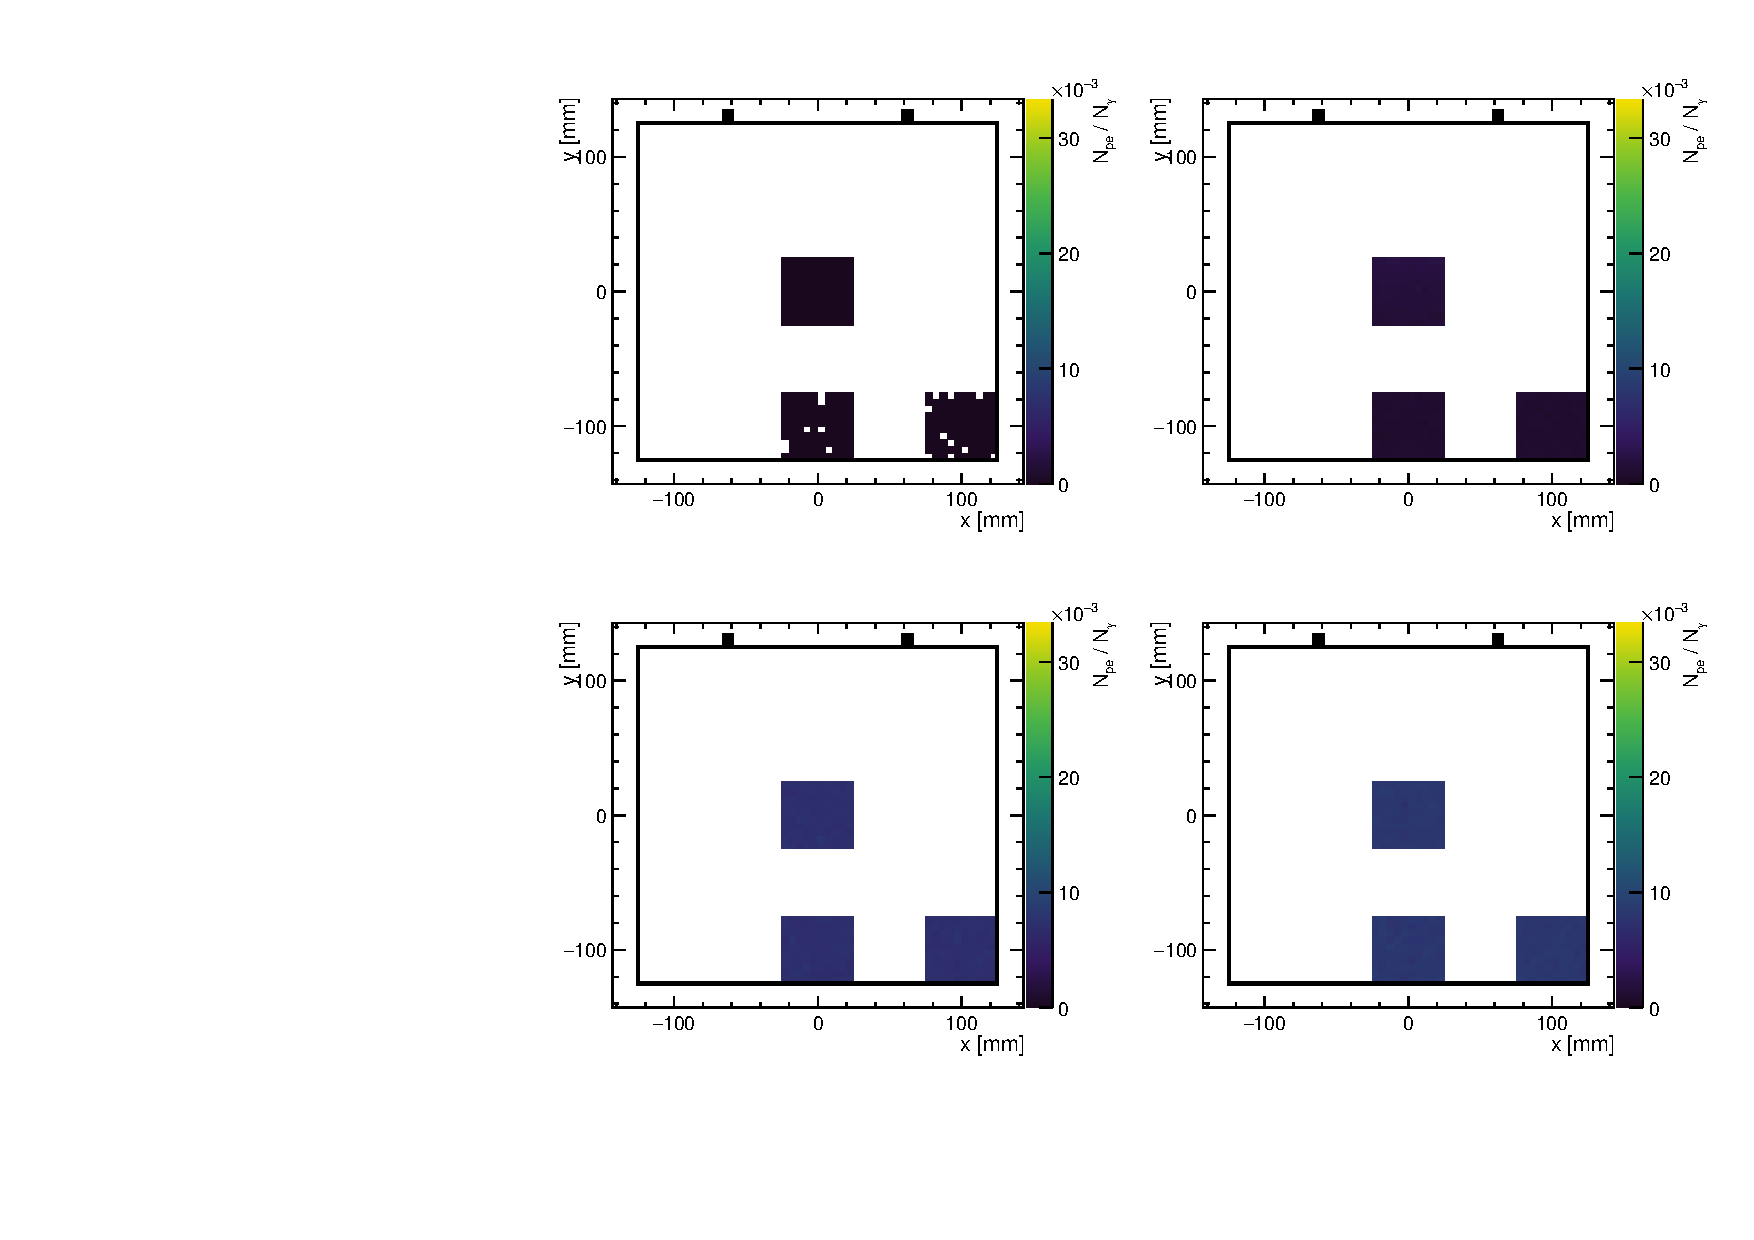
\includegraphics[width=\textwidth]{figures/efficiency_grid_cfg3_all.pdf}
\caption{Collection efficiency map, config~3 (2 SiPMs, both on the top $+y$ side).
Black squares mark the SiPM positions.}
\label{fig:grid3}
\end{figure}

\begin{figure}[H]
\centering
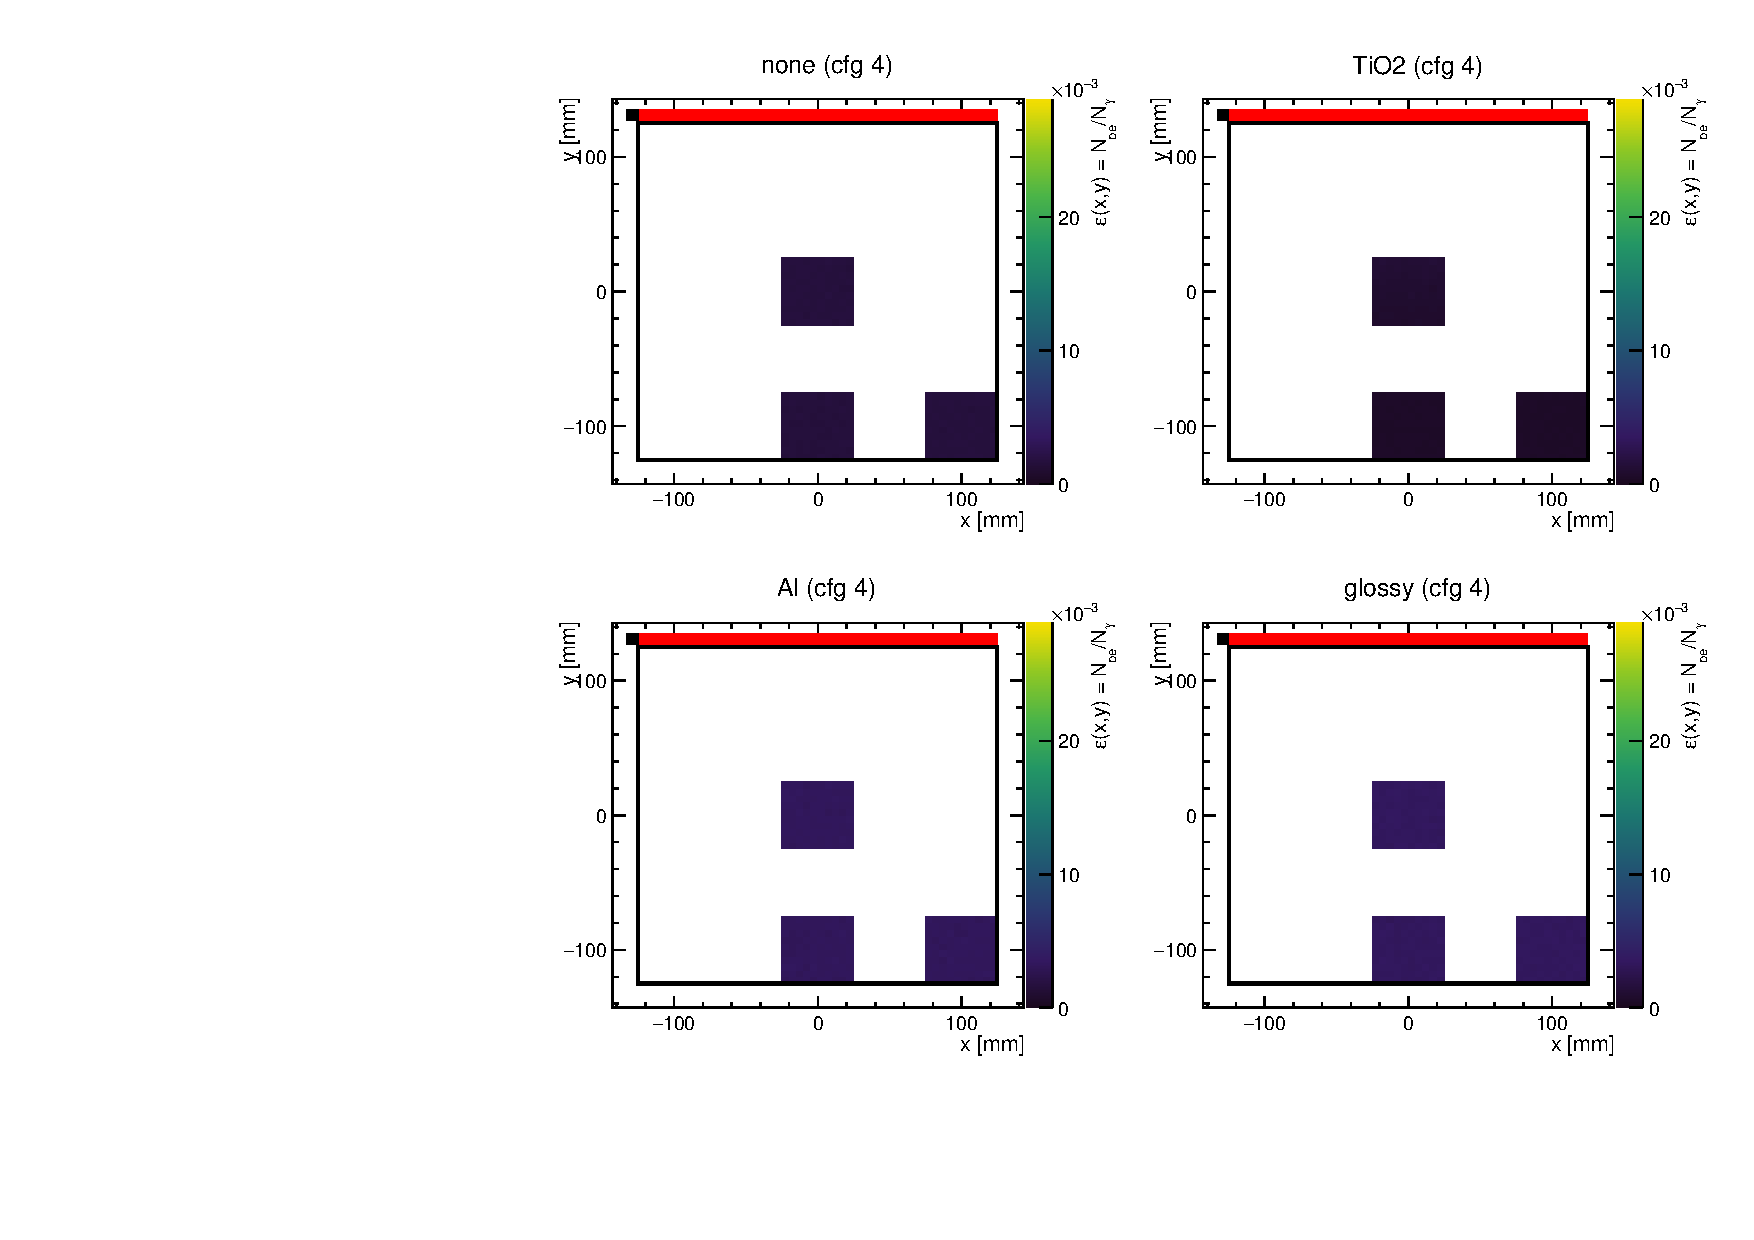
\includegraphics[width=\textwidth]{figures/efficiency_grid_cfg4_all.pdf}
\caption{Collection efficiency map, config~4 (single SiPM $+$ WLS fibre clamp).
The black square marks the read-out SiPM at the top-left corner; the clamp runs
along the top edge. Same report frame and binning as Figs.~\ref{fig:grid1}--\ref{fig:grid3}.}
\label{fig:grid4}
\end{figure}

\begin{table}[H]
\centering
\caption{Position dependence of the collection efficiency, config~1 (all
SiPMs). Each beam patch is \SI{50}{\milli\meter}$\times$\SI{50}{\milli\meter}
and lies fully on the plate, so the produced-photon denominators are equal.}
\label{tab:positions}
\small
\begin{tabular}{@{}lccc@{}}
\toprule
Reflector & Centre & Edge & Corner \\
\midrule
Bare   & $1.7\times10^{-4}$ & $1.3\times10^{-4}$ & $2.8\times10^{-4}$ \\
TiO$_2$& $7.3\times10^{-3}$ & $9.1\times10^{-3}$ & $1.27\times10^{-2}$ \\
Al     & $2.70\times10^{-2}$ & $2.61\times10^{-2}$ & $2.60\times10^{-2}$ \\
Glossy & $3.04\times10^{-2}$ & $2.97\times10^{-2}$ & $2.96\times10^{-2}$ \\
\bottomrule
\end{tabular}
\end{table}

% =====================================================================
\section{Whole-slab irradiation}
\label{sec:whole}
% =====================================================================

The matrix scan illuminates only three \SI{50}{\milli\meter}$\times$\SI{50}{\milli\meter}
patches, so it resolves the light collection at the centre, edge and corner but
not the full plate. To obtain a complete position-resolved map we ran a second,
\emph{whole-slab} configuration: the GPS plane is expanded to
$250 \times \SI{250}{\milli\meter}$ (\texttt{halfx} $=$ \texttt{halfy} $=$
\SI{125}{\milli\meter}), so the primary muon's first-entry position is sampled
\emph{uniformly} over the entire plate. Ten thousand events are generated per
(config, reflector); the efficiency is reconstructed from the same
\texttt{sipmHits} tree, in $10 \times \SI{10}{\milli\meter}$ cells, as
\[
  \varepsilon(x,y) = \frac{\sum_{e\,\in\,\text{cell}} \pe^{(e)}}
                          {\sum_{e\,\in\,\text{cell}} \ngam^{(e)}},
\]
i.e.\ identically to Eq.~\ref{eq:eff} but binned in the entry position. Because
the beam now covers the whole plate, the whole-slab maps fill in the gaps left
by the three-patch scan.

Figure~\ref{fig:wholeslab} shows the complete set of full-plate maps for
config~1, one panel per reflector. For the bare plate, averaged over the whole
surface the efficiency is $\varepsilon = 4.7\times10^{-4}$, consistent with the
three-patch bare values of Table~\ref{tab:positions}. The map reveals a clear
radial structure that the three discrete patches could only hint at: the
efficiency is lowest at the centre ($\varepsilon \approx 1.8\times10^{-4}$ within
$r < \SI{60}{\milli\meter}$) and rises monotonically toward the edges
($\varepsilon \approx 5.4\times10^{-4}$ in the outer region), i.e.\ by roughly a
factor of three. This is exactly the signature of edge readout combined with
frustrated-TIR absorption: photons created near a sensor-bearing face have a
short path to detection, whereas photons born at the centre must random-walk to
an edge through the lossy holder contact, and most are absorbed before
arriving.

The reflective panels show the same ordering as the matrix scan, with the
position dependence progressively erased. TiO$_2$ is about twenty times brighter
than the bare plate ($\varepsilon = 1.08\times10^{-2}$) and its centre-to-edge
gradient is much weaker ($7.7\times10^{-3}$ for $r < \SI{60}{\milli\meter}$
versus $1.15\times10^{-2}$ beyond, a factor of $\sim\!1.5$). Al is brighter again
($2.69\times10^{-2}$) and almost perfectly \emph{flat}: the centre
($2.67\times10^{-2}$) equals the outskirts ($2.70\times10^{-2}$). Glossy is the
brightest ($3.04\times10^{-2}$) and likewise flat ($3.03$ vs.\
$3.05\times10^{-2}$). Diffuse recycling (TiO$_2$) and specular mixing (Al,
glossy) both reduce the penalty of being far from a sensor, the specular mirrors
so thoroughly that the entry position is effectively erased, whereas the bare
plate---whose frustrated TIR leaks into the holder---retains a steep edge
gradient.

\begin{figure}[H]
\centering
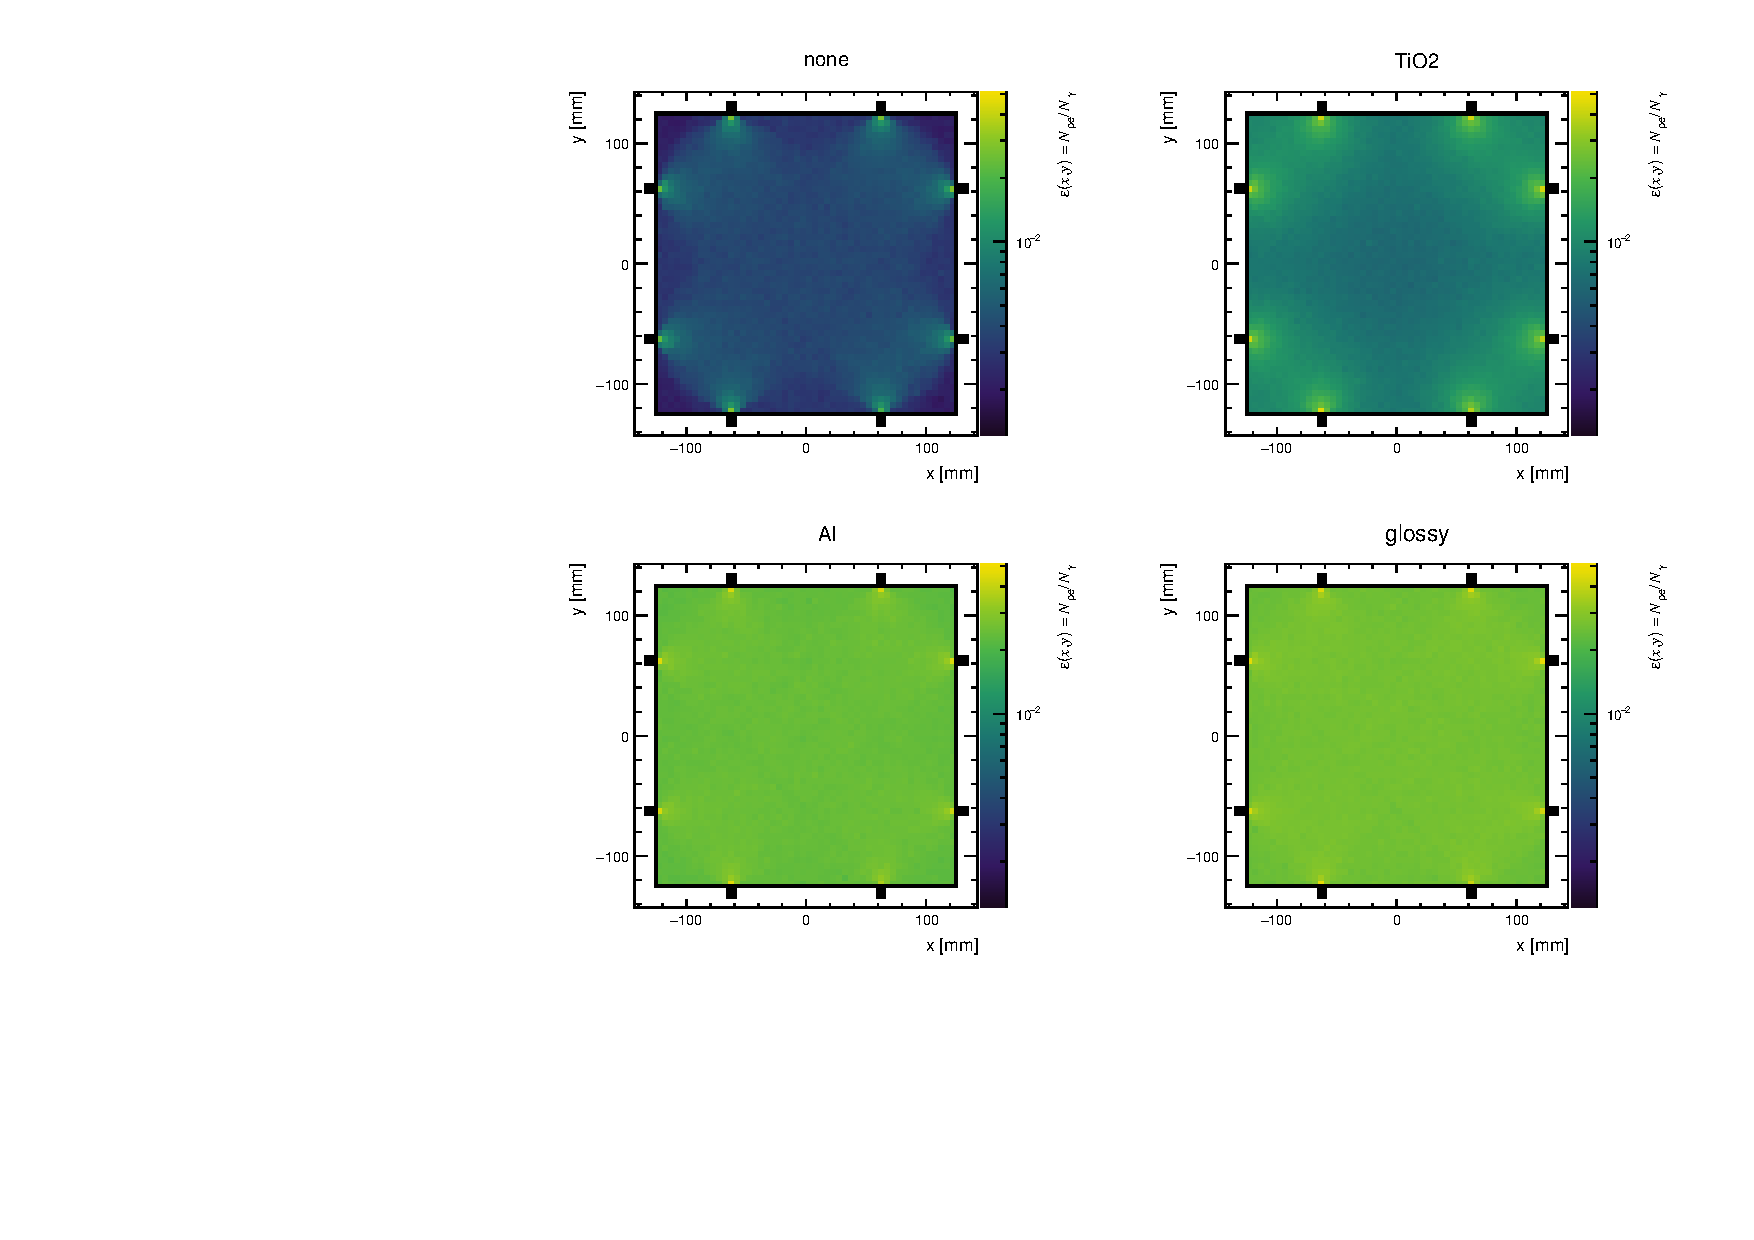
\includegraphics[width=\textwidth]{figures/whole_slab_cfg1.pdf}
\caption{Full-plate collection-efficiency maps for config~1, from \num{10000}
whole-slab events per panel ($10 \times \SI{10}{\milli\meter}$ cells, on a
logarithmic colour scale shared by the panels). Bare plate (top left) rises from
the centre toward the instrumented edges; TiO$_2$ (top right) is roughly twenty
times brighter with only a weak gradient; Al (bottom left) and glossy (bottom
right) are brighter still and almost flat. The bold rectangle is the
\SI{250}{\milli\meter}$\times$\SI{250}{\milli\meter} slab outline and the black
squares mark the eight SiPM positions.}
\label{fig:wholeslab}
\end{figure}

Figure~\ref{fig:wholeslab2} repeats the whole-slab scan for config~2 (four
sensors, one on each lateral face at the config-1 offsets). Every configuration
is weaker than
its config-1 counterpart---roughly halved, as expected from the reduced sensor
area---while the reflector ordering and the flattening behaviour are unchanged.
The bare plate gives $\varepsilon = 2.6\times10^{-4}$ with the same strong edge
gradient ($1.3\times10^{-4}$ at the centre versus $2.9\times10^{-4}$ outside
$r = \SI{60}{\milli\meter}$); TiO$_2$ reaches $5.55\times10^{-3}$ with a milder
gradient, and Al and glossy reach $1.42\times10^{-2}$ and
$1.62\times10^{-2}$, both nearly flat. The monotone bare $\ll$ TiO$_2$ $<$ Al
$\approx$ glossy sequence and the progressive erasure of the position dependence
are therefore robust against the sensor count: fewer sensors lower the overall
light collection but do not change the physics of the wrapper.

\begin{figure}[H]
\centering
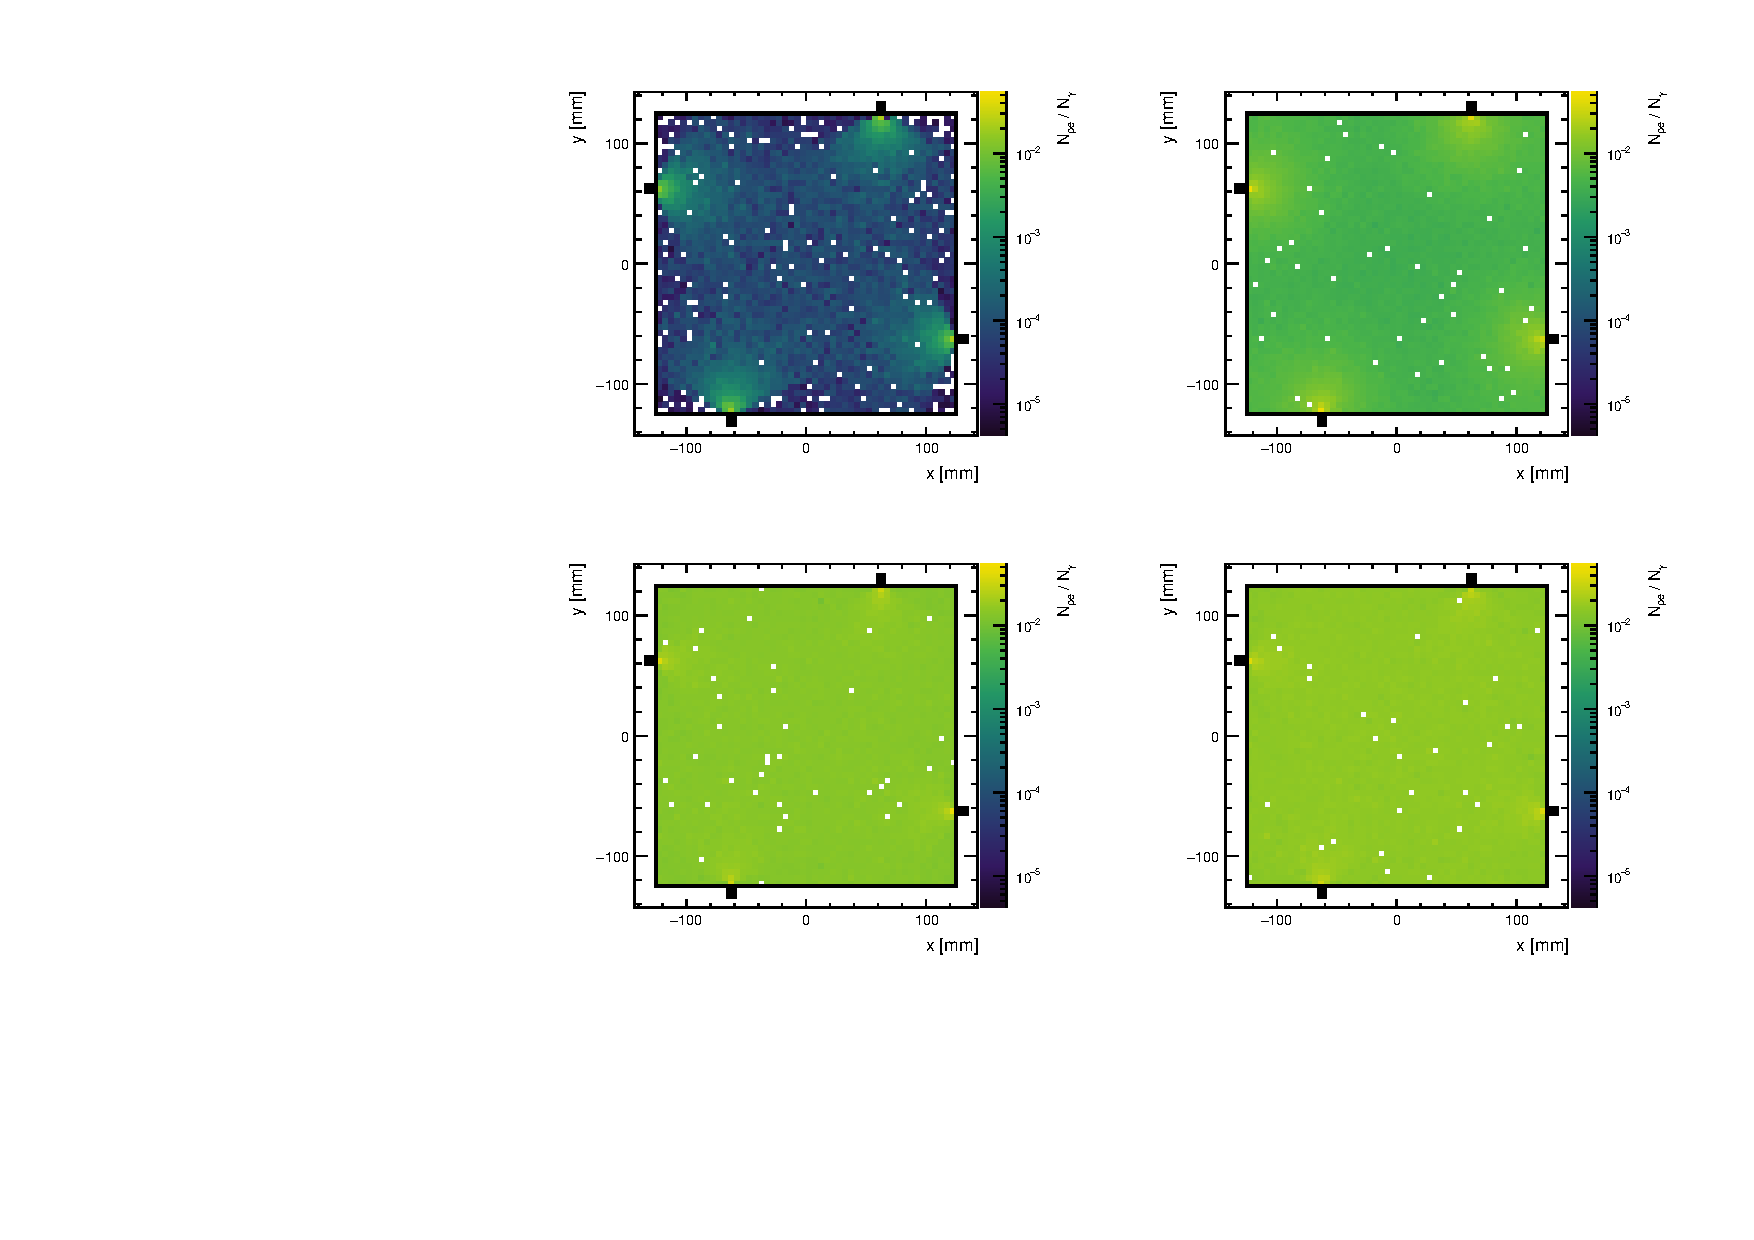
\includegraphics[width=\textwidth]{figures/whole_slab_cfg2.pdf}
\caption{Full-plate collection-efficiency maps for config~2 (four SiPMs, one per
lateral face at the config-1 offsets), otherwise identical to
Fig.~\ref{fig:wholeslab}. The reflector
ordering and the centre-to-edge flattening are the same, with each efficiency
about half the config-1 value.}
\label{fig:wholeslab2}
\end{figure}

Finally, Fig.~\ref{fig:wholeslab3} shows config~3, in which both sensors sit on
the same (top, $+y$) face. The integrated efficiencies are the lowest of the
direct-coupled
configurations---bare $1.1\times10^{-4}$, TiO$_2$ $2.7\times10^{-3}$, Al
$7.2\times10^{-3}$, glossy $8.2\times10^{-3}$---because concentrating both
sensors on one face halves the solid angle available to photons born on the
opposite side. The maps make the resulting asymmetry visible: the bare and
TiO$_2$ panels are brightest near the instrumented top ($+y$) edge and dimmest on
the far ($-y$) side ($4.4\times10^{-5}$ at the centre versus $1.3\times10^{-4}$
outside $r = \SI{60}{\milli\meter}$ for the bare plate). The specular wrappers
again homogenise the response, with Al and glossy flat to better than 1\%
between the inner and outer regions.

The whole-slab irradiation was carried out for the direct-coupled layouts only
(configs~1--3); the WLS-fibre layout (config~4) is still under development and
has no full-plate run. Across the three direct-coupled layouts the
reflector ordering is identical and monotone,
\[
\text{bare} \;\ll\; \text{TiO}_2 \;<\; \text{Al} \;<\; \text{glossy},
\]
and the efficiency scales roughly with the collected photosensitive area,
confirming that the wrapper, not the readout layout, governs the collection
efficiency.

\begin{figure}[H]
\centering
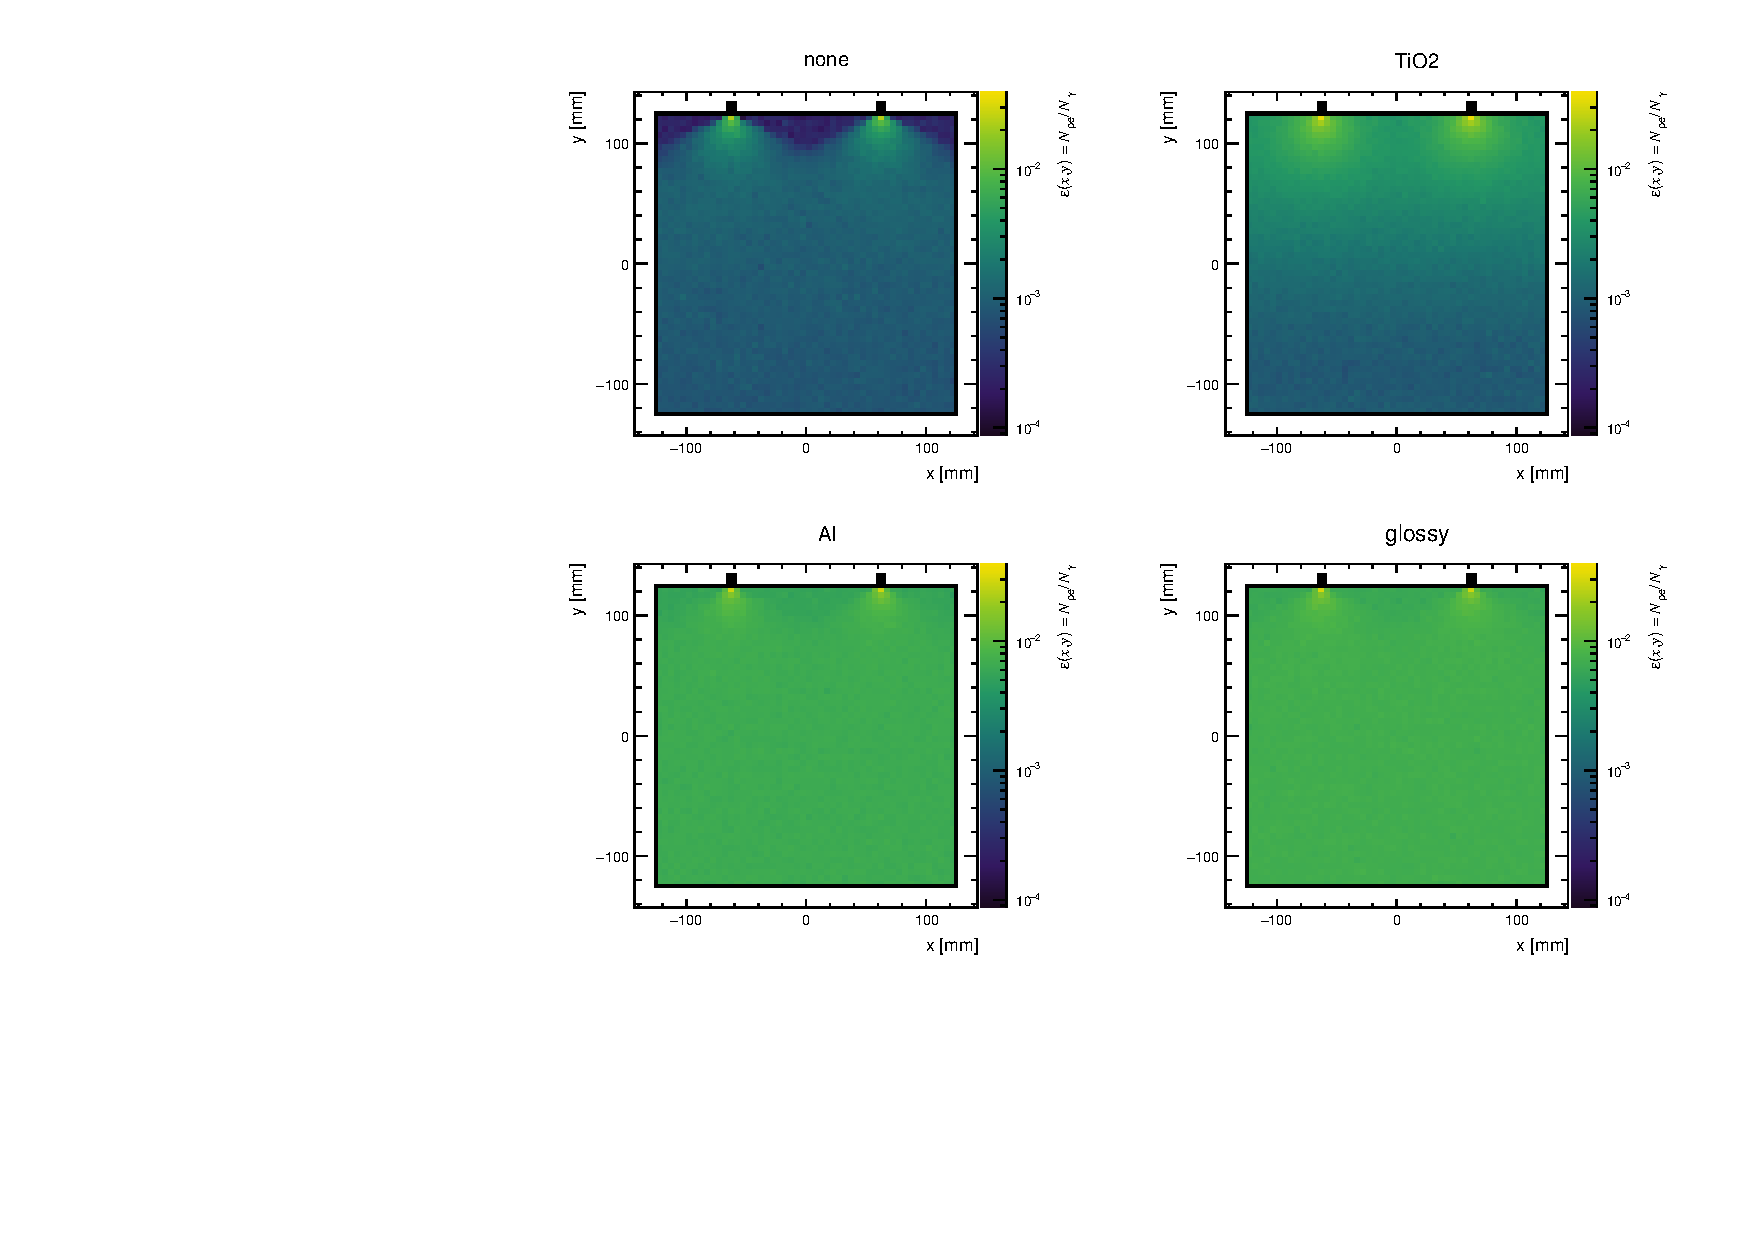
\includegraphics[width=\textwidth]{figures/whole_slab_cfg3.pdf}
\caption{Full-plate collection-efficiency maps for config~3 (two SiPMs, both on
the top $+y$ face). The lowest efficiencies of the direct-coupled layouts and the
clearest top--bottom asymmetry appear here; the specular wrappers (Al, glossy)
again flatten the response.}
\label{fig:wholeslab3}
\end{figure}

% =====================================================================
\section{Caveats and open items}
\label{sec:caveats}
% =====================================================================

\paragraph{Intermittent multi-threaded stall.}
During the matrix production runs a rare stall was observed: on one occasion a
single worker thread entered a tight loop (100\% CPU) while the remaining
threads waited at the event-level barrier, freezing the run. The condition is
intermittent---the same macro completed normally on a clean re-run---and is
consistent with a pathological optical track (e.g.\ a photon bouncing in a
near-degenerate configuration) rather than a deterministic defect. Because a
single stalled task would consume the entire wall-time allocation on a batch
system, the production workflow wraps every task in a timeout with automatic
retry. The matrix results reported here are unaffected: all 48 files completed
(four layouts $\times$ four reflectors $\times$ three positions), and the frozen
run was discarded and regenerated.

\paragraph{Reversed position trend in TiO$_2$.}
For the mirror-like wrappers (Al, glossy) the response is essentially flat across
the three patches (contrast $<\!\SI{9}{\percent}$, Table~\ref{tab:contrast}),
with the centre marginally the most efficient and the corner the least, consistent
with the shortest average path to a sensor. The TiO$_2$ configuration instead
shows a clear corner $>$ edge $>$ centre ordering (a factor \num{1.7}). Since \texttt{groundfrontpainted} is purely
Lambertian (no TIR, no specular reflection), the sharp corner provides two
orthogonal painted walls close to the sensor-bearing edges, and diffusely
scattered light is re-emitted into the plate rather than specularly returned;
the corner geometry can therefore couple more light into the edge sensors. The
effect persists at the higher \num{1000}-event-per-position statistics used
here, though no corresponding trend is reported in Ref.~\cite{Rao2025} and it
should be confirmed with independent simulation settings before being
interpreted physically.

\paragraph{Scale and normalisation.}
The absolute efficiencies are model-dependent: they are fixed by the assumed
PDE curve, the grease coupling, and the absorbed-fraction of the tabulated
reflectivities. The robust result is the \emph{ordering} and the qualitative
splitting into an effectively absorbing bare case and a reflective family.

% =====================================================================
\section{Summary}
% =====================================================================

A \gfour\ optical simulation of a \SI{250}{\milli\meter}$\times$\SI{250}{\milli\meter}$\times$\SI{10}{\milli\meter} polished plastic
scintillator read out by side-mounted SiPMs has been developed and applied to a
full matrix of four SiPM layouts and four reflector treatments at three beam
positions. The optical physics---unified surface model, finish selection,
photocathode PDE via the boundary process, and per-event photon
accounting---has been verified against the \gfour\ source. The results reproduce
the experimentally observed ordering
$\text{bare} \ll \text{TiO}_2 < \text{Al} \approx \text{glossy}$, with the bare
plate suppressed by two to three orders of magnitude by frustrated total internal
reflection into a black holder. A complementary whole-slab irradiation samples
the full \SI{250}{\milli\meter}$\times$\SI{250}{\milli\meter} plate uniformly and
yields a complete collection-efficiency map, which for the bare configuration
shows the expected factor-of-three rise from centre to edge. Keeping the three
irradiation patches separate---rather than collapsing them to a single beam-axis
radius---reveals that the reflective wrappers homogenise the response: the
position contrast stays below \SI{9}{\percent} in every layout, and the per-sensor
light sharing becomes nearly uniform, whereas the bare plate concentrates
\SI{91}{\percent} of the collected light on the two sensors nearest the beam.

\begin{thebibliography}{9}
\bibitem{Rao2025} Rao \emph{et al.}, J.~Appl.\ Phys.\ \textbf{138}, 114504 (2025).
\bibitem{G4OpticalPhysics} \gfour\ Collaboration, \emph{Physics Reference Manual: Optical Processes}, Geant4 v11.3.2.
\bibitem{EJ200} Eljen Technology, \emph{EJ-200 General Purpose Plastic Scintillator} datasheet.
\bibitem{UPS923A} Amcrys, \emph{UPS-923A Plastic Scintillator} datasheet.
\bibitem{Birks1970} J.~B.~Birks and F.~A.~Craun, \emph{The theory and practice of scintillation counting} (1970).
\end{thebibliography}

\end{document}
